 % Żeby nie było syfu to kolejne sekcje dodajemy do chapters/
% A potem includujemy za pomocą \input{chapters/...}

% Używamy \( \) i \[ \] zamiast dolarów -- tak jak się robi w LaTeXu


\documentclass[12pt, a4paper, polish, openany]{book}

% Please, let's familiarize ourselves with notatki.sty and tcs.sty so that we don't reinvent the wheel
\usepackage{notatki}
\fancyhead[L]{\textbf{\textit{MO}}}

\raggedbottom

\begin{document}

% Front page and table of contents
\frontmatter

\begin{titlepage} 
    \begin{center}
         \begin{figure}[h]
            \centering
            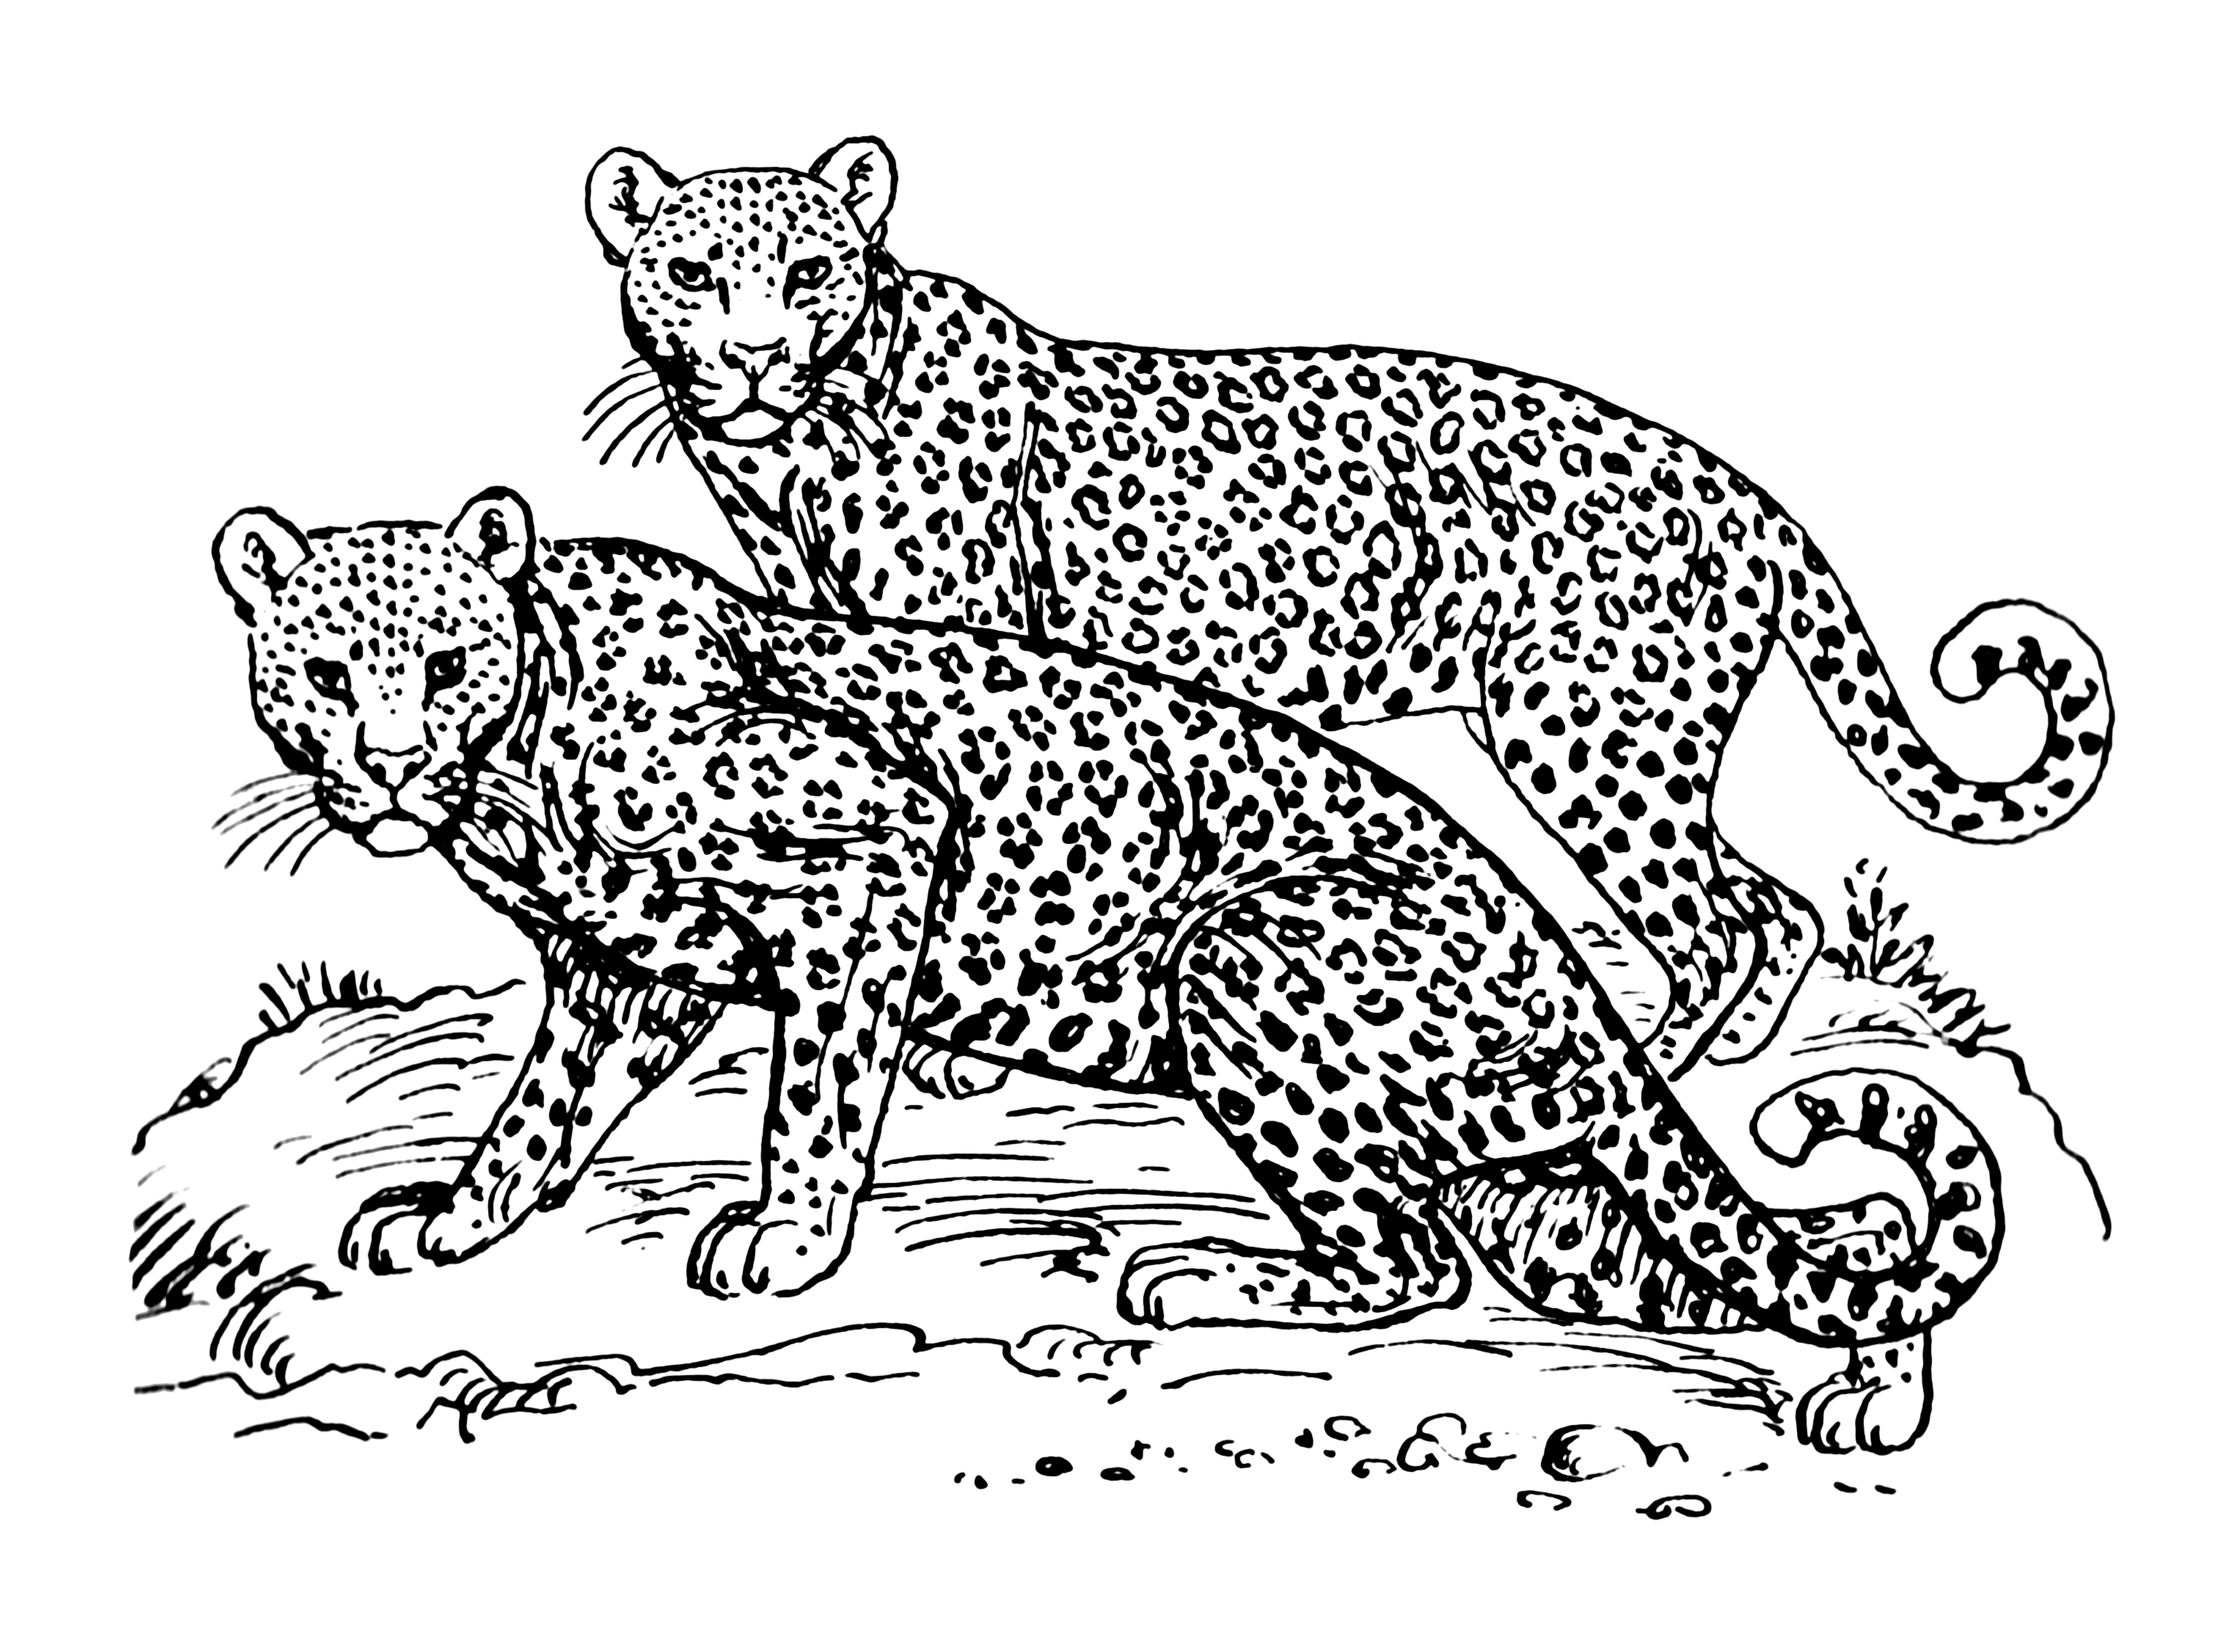
\includegraphics[]{img/pumy.png}
           
        \end{figure}
        
        \Huge
        \textbf{\textsc{Metody Probabilistyczne \\ w Uczeniu Maszynowym}}
        
        \vspace{0.5cm}
        \Large
        \textsc{Zagadnienia Egzaminacyjne}
        \line(1,0){330}
        
        \normalsize
        
        \vspace{1cm}
        \textit{,,Gdzie błąd?''}
        \vspace{1cm}

        \textit{\textsc{Popełnione przez}}\\
        \vspace{5mm}
  
        \textbf{\textsc{Załatany Ponton}}
 
        \vfill

        Kraków \\
        Anno Domini 2023
    \end{center}
\end{titlepage}

\tableofcontents
\section*{Licencja}
    \begin{figure}[h]
    	\begin{minipage}[c]{0.25\textwidth}
    		
\includegraphics[width=0.7\textwidth]{licencja.png}
    	\end{minipage}\hfill
    	\begin{minipage}[c]{0.75\textwidth}
    		\caption*{
    			Ten utwór jest dostępny na 
    			\href{https://creativecommons.org/licenses/by-sa/4.0/}{licencji Creative Commons Uznanie autorstwa
    			na tych samych warunkach 4.0 Międzynarodowe.}
    		}
    	\end{minipage}
    \end{figure}


% Actual content
\mainmatter

\chapter*{Podstawy}
\section{Definicje}

\begin{definition}
	Mówimy, że model (przewidujący wyjścia) jest \textbf{liniowy} jeśli jego wyjścia można opisać funkcją
	\[
		f_\theta(x) = \theta_0 + \sum_{i=1}^k \theta_i \cdot \phi_i(x_i)
	\]
	gdzie funkcje \( \varphi_i \) są dowolne i nazywamy je \textbf{funkcjami bazowymi}.
\end{definition}

Zauważmy, że model jest liniowy pod względem parametru \( \theta \) a nie względem \( x \). Używając odpowiednich funkcji bazowych możemy opisywać funkcje \( f \) które nie są funkcjami liniowymi.

\chapter{Języki regularne}
\section{Teza Churcha}

\textbf{Teza Churcha} jest nieformalną tezą głoszącą, że jakaś funkcja matematyczna z liczb naturalnych może być policzona za pomocą \textit{efektywnej metody} (to znaczy takiej, którą można w jakiś sposób w pełni zautomatyzować) wtedy i tylko wtedy gdy może być obliczona przez Maszynę Turinga. 

W pierwszej połowie XX wieku próbowano sformalizować pojęcie \textbf{funkcji obliczalnych}, w związku z czym powstały 3 sformalizowane modele obliczeń:

\begin{enumerate}
    \item Rachunek \(\lambda\)
    \item Funkcje pierwotnie rekurencyjne
    \item Maszyny Turinga
\end{enumerate}

Okazuje się, że funkcja jest \(\lambda\)-obliczalna wtedy i tylko wtedy gdy jest pierwotnie rekurencyjna, oraz że jest pierwotnie rekurencyjna wtedy i tylko wtedy gdy jest obliczalna przez Maszynę Turinga.

Z racji równoważności tych trzech modeli obliczeń ludzie doszli do wniosku, że być może nie ma lepszego sposobu na automatyczne obliczanie funkcji. 
\section{Maszyna Turinga}

\begin{definition}

 \textbf{Maszyna Turinga} to tupla
    \[
        MT = (Q, \Sigma, \Gamma, \delta, q_0, \blank, F)
    \]
    gdzie
    \begin{itemize}
        \item \( Q \) -- skończony zbiór stanów
        \item \( \Sigma \subseteq \Gamma \) -- skończony alfabet wejściowy
        \item \( \Gamma \) -- skończony alfabet taśmowy
        \item \( \delta : Q \times \Gamma \rightarrow 
        Q \times \Gamma \times \set{-1, +1}
        \) -- stan, litera \( \rightarrow \) nowy stan, zmiana litery, ruch głowicą (lewo, prawo)
        \item \( q_0 \) -- stan startowy
        \item \( \blank \in \Gamma \setminus \Sigma \) -- pusty symbol / zero (domyślny symbol taśmy)
        \item \( F \) -- zbiór stanów akceptujących
    \end{itemize}
    
    Ponadto zakładamy, że \(Q \cap \Gamma = \varnothing\). 
\end{definition}

\begin{definition}
    \textbf{Opis chwilowy} (konfiguracja) Maszyny Turinga to słowo nad językiem \(\Gamma^* q\Gamma \Gamma^* \). 
\end{definition}

\begin{definition}
    Konfiguracja startowa Maszyny Turinga to słowo postaci \(q_0w\blank\).
\end{definition}

\begin{definition}
    Definiujemy relację \( \vdash_M \) na konfiguracjach MT.
    
    Przejście w lewo ,,wewnątrz taśmy'':
    \[
        \alpha A q B \beta 
        \vdash_M
        \alpha q' A B' \beta
    \]
    
    gdzie \(\alpha, \beta \in \Gamma^*\), \(A, B \in \Gamma\), \(q, q'\in Q\), oraz \(\delta(q, B) = (q', B', -1)\).
    
    Analogicznie definiujemy przejście w prawo ,,wewnątrz taśmy'':

       \[
        \alpha q B \beta 
        \vdash_M
        \alpha B' q' \beta
    \]
    
    gdzie \(\alpha, \beta \in \Gamma^*\), \(B \in \Gamma\), \(q, q'\in Q\), oraz \(   \delta(q, B) = (q', B', 1) \).
    
    Definiujemy również ,,skrajne'' przejścia -- przejście w prawo ,,na skraju taśmy'':
    
    \[ 
        q B 
        \vdash_M
        B' q' \blank 
    \]
    
    gdzie \(B, B' \in \Gamma\), \(q, q' \in Q\), oraz \( \delta(q, B) = (q', B', 1) \)

    Przejście w lewo ,,na skraju taśmy'':
    \[
         q B 
        \vdash_M
        q' \blank B' 
    \]
    
    gdzie \(B, B' \in \Gamma\), \(q, q' \in Q\), oraz \( \delta(q, B) = (q', B', -1)\)

    
\end{definition}


\begin{definition}
    \textbf{Język akceptowany przez Maszynę Turinga} definiujemy jako
    \[
        L(M) = \set{w \in \Sigma^* \mid \exists_{q_f \in F} \exists_{\alpha, \beta \in \Gamma^*} q_0w\blank \vdash_M^* \alpha q_f \beta}
    \]
\end{definition}

\begin{theorem}
    Maszyny Turinga nie wolno nazywać ,,automatem''.
\end{theorem}
\begin{proof}
    Maszyna Turinga jest narzędziem dużo potężniejszym niż godne pogardy poznane dotychczas automaty. Dlatego należy się jej odpowiedni szacunek.
\end{proof}
\begin{corollary}
    Nazwanie Maszyny Turinga ,,automatem'' skutkuje skreśleniem z~listy studentów.
\end{corollary}
\section{Niedeterministyczna Maszyna Turinga}

\subsection{Definicja}

\begin{definition}
	Niedeterministyczną Maszynę Turinga definiujemy tak samo jak deterministyczną Maszynę Turinga, przy czym funkcja \( \delta \) zostaje relacją; ciągnie to za sobą dosyć oczywiste konsekwencje w definiowaniu relacji \( \vdash\).

	Co ciekawe, definicja języka akceptowanego się nie zmienia; nadal zwyczajnie chcemy mieć stan akceptujący w domknięciu przechodnim.
\end{definition}

\subsection{Równoważność z deterministyczną Maszyną Turinga}

\begin{theorem}
	Następujące stwierdzenia są równoważne dla dowolnego języka \( L \subset \Sigma^*\):
	\begin{enumerate}
		\item Istnieje deterministyczna Maszyna Turinga DM taka, że \(L(DM) = L\).
		\item Istnieje niedeterministyczna Maszyna Turinga NM taka, że \(L(NM) = L \).
	\end{enumerate}
\end{theorem}

\begin{proof}
	Dowód faktu, że mając deterministyczną Maszynę Turinga możemy utworzyć niedeterministyczną Maszynę Turinga jest trywialny (każda funkcja jest relacją).

	Skupmy się zatem na dowodzie w drugą stronę; mamy daną niedeterministyczną Maszynę Turinga \(N\) i chcemy stworzyć równoważną deterministyczną Maszynę Turinga \(M\). Aby to uczynić, będziemy (intuicyjnie) chodzić BFS-em po nieskończonym grafie konfiguracji maszyny \(N\).

	Formalizacja tego jest bardzo ciężka, mimo faktu że idea jest prosta (zatem podamy ideę). W alfabecie chcemy mieć jakiś separator, który jedyne do czego będzie używany, to do rozpatrywania kolejnych konfiguracji ,,w kolejce''.

	Na początku ,,w kolejce'' konfiguracji do analizy mamy jedynie konfigurację startową. Mając głowicę w jakimś położeniu, znając jej stan i to co jest ,,na prawo'' od niej, dopisujemy do kolejki symbol separacji konfiguracji, a następnie całą naszą konfigurację po wykonanym którymś przejściu z maszyny \(N\). Procedurę tę wykonujemy dla każdego możliwego przejścia z \(N\).

	Gdy ,,przerobimy'' wszystkie możliwe przejścia z \(N\) (dla każdej sytuacji jest ich skończenie wiele, więc zakodowanie tego jak \(M\) ma się zachowywać by wygenerować wszystkie te konfiguracji jest osiągalne), przechodzimy do następnej konfiguracji z~kolejki. No BFS, co tu jeszcze można powiedzieć?

	Za każdym razem, gdy analizujemy nową konfigurację, sprawdzamy czy zapisany w niej stan jest akceptujący; jeśli tak, to wtedy akceptujemy słowo. Jeśli nie ma zdefiniowanych przejść dla określonej sytuacji, to nie robimy nic i przechodzimy do kolejnej konfiguracji w kolejce.

	Again, formalizowanie tego wymagałoby wprowadzenia dodatkowych stanów które trzymałyby informacje o tym, co ,,widzi'' maszyna \(N\); ponadto wszystkie stany maszyny \(N\) muszą wejść do alfabetu taśmowego maszyny \(M\) by móc je również trzymać taśmie. To wszystko jest wykonywalne, ale przykre w implementacji.
\end{proof}

\section{k-taśmowa maszyna Turinga}

Jest równoważna zwykłej maszynie. Czemu ? Bo możemy trzymać wszystkie taśmy szeregowo na jednej taśmie. Aby zrobić przejście przechodzimy od lewej do prawej po całej taśmie i zbieramy informacje o położeniu i stanach głowic -- następnie wykonujemy odpowiednie przejścia rozszerzając przy tym reprezetancje taśm jeśli trzeba.


\section{PDA z k stosami}

Okazuje się że jeśli dodamy PDA drugi stos to jest on równoważny Maszynie Turinga -- pierwszego stosu będziemy używali jako taśmy, drugiego będziemy używali jako bufor aby móc dowolnie przeglądać i modyfikować pierwszy stos.


\section{Uniwersalna Maszyna Turinga}

Maszyny Turinga są super, ale czy taka maszyna potrafi zasymulować jakąś inną, być może dowolną maszynę? Otóż okazuje się że tak -- umiemy skonstruować taką Maszynę Turinga, która jak dostanie na wejściu zakodowaną Maszynę Turinga \( M \) oraz jej wejście \( w \) to będzie w stanie zasymulować zachowanie \( M \) na \( w \) i zwrócić (zakodowany w tym samym formacie co wejście) wynik symulacji.

Niech \( M = (Q, \Sigma, \Gamma, \delta, q_0, \blank, F) \) będzie (deterministyczną) maszyną którą chcemy symulować. Pokażemy jak zakodować \( M \) nad alfabetem \( \Sigma_U = \set{0, 1} \).

\begin{itemize}
	\item Niech \( Q = \set{q_1, \dots, q_n} \)

	      Kodujemy \( q_i \) jako ciąg \( i \) jedynek.

	\item \( \blank \) będziemy kodować jako pojedynczą jedynkę.


	\item Podobnie niech \( \Sigma = \set{a_1, \dots, a_n} \)

	      Kodujemy \( a_i \) jako ciąg \( i + 1 \) jedynek.

	\item Dla \( \Gamma = \set{z_1, \dots z_n} \)

	      Kodujemy \( z_i \) jako ciąg \( i + \card{\Sigma + 1} \) jedynek -- dla odróżnienia od \( \Sigma \).

	\item \( \delta \) jest funkcją, czyli zbiorem par \( ((q_1, z_1), (q_2, z_2, \pm 1) \)

	      Parę \( ((q_i, z_j), (q_k, z_l), 1) \) zakodujemy jako

	      \[
		      \underbrace{1 \dots 1}_i
		      0
		      \underbrace{1 \dots 1}_j
		      0
		      \underbrace{1 \dots 1}_k
		      0
		      \underbrace{1 \dots 1}_l
		      0
		      1
	      \]

	      Natomiast parę \( ((q_i, z_j), (q_k, z_l), -1) \) zakodujemy jako

	      \[
		      \underbrace{1 \dots 1}_i
		      0
		      \underbrace{1 \dots 1}_j
		      0
		      \underbrace{1 \dots 1}_k
		      0
		      \underbrace{1 \dots 1}_l
		      0
		      11
	      \]

	      Całą deltę kodujemy kodując wszystkie jej pary (w dowolnej kolejności) i oddzielając je dwoma zerami.

	\item \( F = \set{q_{i_1}, \dots q_{i_n}} \) kodujemy jako
	      \[
		      \underbrace{1 \dots 1}_{i_1} 0 \dots 0 \underbrace{1 \dots 1}_{i_n}
	      \]
\end{itemize}

Całą maszynę \( M \) zapisujemy wpisując \( \delta, q_0, F \) oddzielając je ciągiem \( 000 \).

Słowo \( w = a_{i_1} \dots a_{i_n} \) kodujemy jako
\[
	\underbrace{1 \dots 1}_{i_1} 0 \dots 0 \underbrace{1 \dots 1}_{i_n}
\]

Teraz musimy jeszcze powiedzieć jak kodujemy konfigurację maszyny \( M \) a robimy to dość prosto --
Konfigurację \( X_1 \dots X_k q_i X_{k+1} \dots X_n \) kodujemy jako
\[
	0\underbrace{1 \dots 1}_{\text{kod } X_1} 0 \underbrace{1 \dots 1}_{\text{kod } X_k} 00 \underbrace{1 \dots 1}_{\text{kod } q_i} 00 \underbrace{1 \dots 1}_{\text{kod } X_{k + 1}} 0 \underbrace{1 \dots 1}_{\text{kod } X_n} 0
\]

Możemy założyć, że kodowanie \( M \) jest zapisane na taśmie wejściowej po której nigdy nie piszemy, zaś konfigurację \( M \) będziemy trzymać na osobnej taśmie.

Krok symulacji przebiega teraz następująco:
\begin{enumerate}
	\item Zlokalizuj głowicę \( M \) (szukamy \( 00 \))
	\item Znajdź w kodowaniu \( \delta \) wpis odpowiadający przejściu na \( q_i X_k \)
	\item Wykonaj zadane przejście -- możemy wpisać nową konfigurację na osobną, tymczasową taśmę i przepisać ją z powrotem na taśmę na której operujemy.

\end{enumerate}



\section{Przykład konstrukcji CSG i LBA dla prostego języka kontekstowego}

Na ćwiczeniach robiliśmy \( a^nb^nc^n\) który w jednej grupie ćwiczeniowej zajął około 45 minut.\( kmwtw\)

...w innej grupie jednak udało się uporać z tym istotnie szybciej, i przytoczymy to tutaj.

\subsection{LBA}

Automat jest w istocie dość prosty. W każdym kroku głowica wraca na początek, a następnie szuka podciągu \(abc\) (niespójnego!)\
(czyli po prostu przechodzi sprawdzając literki kolejno) jednocześnie oznaczając wykorzystane literki. Jak nie znajdzie, to\
sprawdza czy wszystkie literki są oznaczone (wykorzystane). Jeśli tak to słowo akceptuje, jeśli nie - odrzuca.

\subsection{CSG}

Tu jest istotnie trudniej. Zaczynamy od wygenerowania słowa \(A^nB^n\), a następnie chcemy przypychać żetony.

\begin{enumerate}
	\item Nieterminal \(A\) może wygenerować żeton, jeśli on nie był wykorzystany, a po lewej nic nie ma, lub jest nieterminal wykorzystany \(A'\).
	\item Generowanie żetonu to produkcja \(A \rightarrow [A', Z_1]\).
	\item Żeton możemy przepychać: jeśli lewy sąsiad ma żeton, to ja mogę go wziąc do siebie (\(A \rightarrow [A, Z_1]\)). Jeśli prawy sąsiad ma żeton,\
	      to znaczy że go oddałem, więc mogę się go u siebie pozbyć: \([A, Z_1] \rightarrow A\).
	\item Jeśli żeton \(Z_1\) dotrze do \(B\), to \(B\) zostaje wykorzystane, a żeton zamienia się w \(Z_2\).
	\item Jeśli żeton \(Z_2\) dotrze do ostatniego \(B\), to możemy wygenerować literę \(c\), a żeton znika.
	\item Litery \(a, b\) powstają tylko z \(A', B'\) - czyli wykorzystanych do produkcji C. Oznacza to że nieterminale mogą zniknąć tylko jeśli\
	      wyprodukowaliśmy \(n\) razy \(c\) na końcu (żeton nie może zniknąć inaczej); jednocześnie, nie da się wyprodukować więcej żetonów (więc także literek \(c\)).
\end{enumerate}

\section {Języki rekurencyjnie przeliczalne}

\begin{definition}
	Mówimy że język \( L \) jest \textbf{rekurencyjnie przeliczalny} jeśli istnieje Maszyna Turinga \( M \) taka że \( L(M) = L \).

	Zbiór języków rekurencyjnie przeliczalnych oznaczamy przez \textbf{\( \re \)} (z ang. \textit{Recursively Enumerable}).
\end{definition}

\section {Języki rekurencyjne}

\begin{definition}
	Mówimy, że MT \( M \) ma \textbf{własność stopu} jeśli po skończonej liczbie kroków trafia do jednego z wyróżnionych stanów \( q_{acc}, q_{rej} \) z których jedyne przejścia prowadzą z powrotem do nich samych.
\end{definition}

Powyższa definicja działa zarówno w przypadku deterministycznym (w którym mamy jedną ścieżkę obliczeń) jak i niedeterministycznym (wtedy chcemy żeby każda ścieżka obliczeń miała taką własność).
Niestety formalnie Maszyna Turinga się nie zatrzymuje, ale przyjmujemy że jak już wpadniemy w stan \( q_{acc} \) to akceptujemy słowo i się zatrzymujemy a gdy wpadniemy w stan \( q_{rej} \) to odrzucamy słowo i się zatrzymujemy.

\begin{definition}
	Mówimy że język \( L \) jest \textbf{rekurencyjny} albo \textbf{rozstrzygalny} jeśli istnieje Maszyna Turinga z własnością stopu \( M \) taka że \( L(M) = L \).

	Zbiór języków rekurencyjnych oznaczamy przez \textbf{\( \r \)} (oczywiście z ang. \textit{Recursive}).
\end{definition}
\subsection{Gramatyki typu 0}
Znamy już trochę rodzajów gramatyk, ale każda ma jakieś ograniczenia, które tylko przeszkadzają nam w~generowaniu naprawdę fajnych słów. To właśnie gramatyki typu 0~dadzą nam prawdziwe artystyczne spełnienie. Standardowo mamy
\[
    G = \pars{N, \Sigma, P, S}
\]
przy czym produkcje są w~postaci \(\alpha \rightarrow \beta\), gdzie \(\alpha, \beta \in \pars{N \cup \Sigma}^*\). Prawdopodobnie chcemy też mieć \(\alpha \neq \eps\) --- nie popadajmy w~paranoję, generowanie słów z~pustych ciągów nie ma sensu. Ale ogólnie wygląda na to, że obie strony produkcji mogą być zasadniczo dowolnymi formami zdaniowymi, w~szczególności elementami \(\Sigma^*\). Dla \(\Sigma = \set{a, b}\) może na przykład istnieć produkcja
\[
    aba \rightarrow bb
\]
Ja dalej w~to nie wierzę, ale tak wynikałoby z~definicji, prawda?

Język generowany przez taką gramatykę definiujemy tak, jak już to wielokrotnie widzieliśmy --- możemy podmieniać ciągi zgodnie z~produkcjami i~w~ten sposób tworzyć derywacje.

Co zatem możemy takim cudem wygenerować? Okazuje się, że są to dokładnie języki \(\re\), nie mniej, nie więcej.
\begin{theorem}
    \(L \in \re \iff\) istnieje gramatyka \(G\) typu 0 taka, że \(L\pars{G} = L\)
\end{theorem}
\begin{proof}
    Prowadzimy go oczywiście w~obie strony.
    \begin{itemize}
        \item[\(\impliedby\):] Dostajemy gramatykę typu 0 i~chcemy skonstruować maszynę Turinga, która akceptuje język generowany przez tę gramatykę. Mamy zatem jakieś słowo \(w\) i~chcemy sprawdzić, czy da się je wygenerować. Przypomnijmy sobie, że generowanie to już teraz tylko branie elementów zbioru \(\pars{N \cup \Sigma}^*\) i~podmienianie ich na inne w~większym słowie. Niech więc nasza maszyna Turinga będzie niedeterministyczna i, zaczynając od symbolu \(S\), zwyczajnie zgaduje \emph{co} podmienić i~\emph{na co} podmienić, byle zgodnie z~regułami produkcji. Po każdej takiej podmianie niech sprawdza, czy nie wyszło nam przypadkiem słowo \(w\). Jeśli akurat wyszło, to akceptujemy je --- nasze obliczenie jest dowodem, że da się je wygenerować z~zadanej gramatyki. Wiemy też, że jeśli się da, to któraś ścieżka obliczeń NMT zgadnie ten właściwy sposób. Jeśli zaś \(w \not\in L\pars{G}\), to maszyna Turinga oczywiście nigdy nie zgadnie odpowiedniej derywacji i~nie zaakceptujemy.
        \item[\(\implies\):] Teraz na podstawie maszyny Turinga chcemy skonstruować gramatykę typu 0. Na początku ustalmy pewne założenia na temat otrzymanej maszyny \(M\) --- zaraz przekonamy się, że są całkiem sensowne:
            \begin{itemize}
                \item \(M\) jest jednotaśmowa i~deterministyczna --- wiemy, że każda wielotaśmowa i/lub niedeterministyczna da się do takiej sprowadzić
                \item \(M\) w~jakiś sposób oznacza najdalsze użyte komórki taśmy, z~lewej i~z~prawej --- powiedzmy, że będą to symbole \(\triangleright\) i~\(\triangleleft\) --- gdy taśma się rozszerza, te markery oczywiście mogą być przesuwane, my chcemy tylko móc się zorientować, jaki fragment taśmy został jakkolwiek ruszony
                \item gdy \(M\) znajdzie się w~stanie \(q_f \in F\), czyli zaakceptuje słowo, sprząta jeszcze po sobie --- wymazuje całą taśmę i~przysuwa prawy ogranicznik \(\triangleleft\) do lewego ogranicznika \(\triangleright\)
                \item na koniec przechodzi w~stan \(q_\textrm{done}\), z~którego nie ma już przejść.
            \end{itemize}
            Zatem zakładamy że konfiguracja początkowa naszej maszyny to \(q_0\triangleright w\triangleleft\), natomiast jeśli \(w\) jest akceptowane, to \(M\) zatrzymuje się w~konfiguracji \(\triangleright q_\textrm{done}\triangleleft\). Niby sporo założeń, ale chyba możemy wymagać od maszyny Turinga, że zostawi po sobie jako taki porządek, jeśli nie wpływa to w~żaden sposób na rozpoznawany przez nią język, prawda?
            
            Teraz przechodzimy do fajnego pomysłu: chcemy, aby derywacje w~naszej gramatyce symulowały pracę \(M\) \emph{od końca}. Intuicyjnie, chcemy dojść do słowa \(w \in L\pars{M}\), zaczynając od konfiguracji \(\triangleright q_\textrm{done}\triangleleft\) i~zastanawiając się, jakież to słowo mogło pojawić się na wejściu, że \(M\) zakończyła pracę w~takiej właśnie konfiguracji. Mamy zatem
            \[
                N = \pars{\Gamma \setminus \Sigma} \cup Q \cup \set{S}
            \]
            gdzie \(S\) jest po prostu świeżym symbolem startowym.
            
            Jeśli dla pewnych \(q, q' \in Q, a, a' \in \Gamma\) mamy
            \[
                \delta\pars{q, a} = \pars{q', a', +1}
            \]
            to dodajemy produkcję
            \[
                a'q' \rightarrow qa
            \]
            Widać, że taka produkcja odpowiada za ,,wycofanie'' przejścia w~prawo.
            
            Podobnie, jeśli dla pewnych \(q, q' \in Q, a, a' \in \Gamma\) mamy
            \[
                \delta\pars{q, a} = \pars{q', a', -1}
            \]
            to \emph{dla każdego} \(c \in \Gamma\) dodajemy
            \[
                q'ca' \rightarrow cqa
            \]
            W~ten sposób umożliwiamy ,,wycofanie'' przejścia w~lewo. Musimy uwzględnić \(c\), ponieważ nie wiemy, co wcześniej było po lewej.
            
            Na koniec dodajemy produkcje
            \begin{align*}
                S &\rightarrow \triangleright q_\textrm{done}\triangleleft\\
                q_0\triangleright &\rightarrow \eps\\
                \triangleleft &\rightarrow \eps
            \end{align*}
            
            Jako że poziom formalizmu tego rozwiązania nie budzi zastrzeżeń, widzimy, że \(M\) akceptuje \(w\) wtedy i~tylko wtedy, gdy istnieje derywacja
            \[
                S \rightarrow_G \triangleright q_\textrm{done} \triangleleft \rightarrow_G^* q_0\triangleright w\triangleleft \rightarrow_G w\triangleleft \rightarrow_G w
            \]
            Dokładnie tego sobie życzyliśmy. Ten dowód wymaga jeszcze dopowiedzenia paru technikaliów, ale z~pewnością gorliwy czytelnik (których, jak wiemy, nie brakuje) poradzi sobie z~nimi bez większych trudności.
            
            Dowiedliśmy tym samym, że gramatyki typu 0 są wystarczające do generowania języków rozpoznawanych przez Maszyny Turinga.
            Można się zastanawiać czy to musi być koniecznie gramatyka typu 0 -- dla niektórych języków nie (bo są proste języki), ale dla niektórych języków okazuje się że tak, co dowodzimy biorąc wybrany rodzaj gramatyki i wskazując język akceptowany przez pewną MT, ale niedajacy się wyrazić w tej gramatyce.
            
            
    \end{itemize}
\end{proof}

\section{Relacje między wariantami maszyn Turinga i gramatykami typu 0}
\section{Związek między funkcjami a językami akceptowanymi przez Maszyny Turinga}

\subsection{Funkcje}

Maszyna Turinga oblicza funkcję \(f\) jeśli mając na wejściu argument, zatrzymuje się mając na wejściu wartość funkcji dla tego argumentu.\
Odpowiada to akceptowaniu języka \((x, f(x))\); istotnie, możemy łatwo skonstruować maszynę rozpoznającą taki język - dla argumentu symuluje\
maszynę obliczającą wartość, i porównuje z podaną wartością. W drugą stronę analogicznie, dla języka z \(\r\) będącego powyższej postaci możemy\
przypomnieć sobie trik z symulowaniem wielu wejść równolegle (patrz: maszyny Turinga dla prostych problemów); w tym przypadku tymi wejściami\
będą nasze wejście oraz zgadywana wartość. Skoro funkcja ma wartość, to w końcu zgadniemy odpowiednią parę która należy do języka.

\subsection{Funkcje częściowe}

Maszyna Turinga oblicza funkcję częściową \(f\) jeśli zachowuje się zastępująco:

\begin{enumerate}
	\item Mając na wejściu argument z dziedziny, zatrzymuje się z wypisaną na taśmie wartością;
	\item Mając na wejściu coś z poza dziedziny, nie zatrzymuje się.
\end{enumerate}

Zależności są podobne jak wyżej, z tym że z klasą \(\re\). Jeśli funkcja dla jakiegoś \(x\) nie jest zdefiniowana, to symulując maszynę obliczającą\
funkcję zawiesimy się - ale to nie problem, bo słowo i tak nie powinno zostać zaakceptowane, a jesteśmy w \(\re\). W drugą stronę również podobnie,\
lecz funkcja może nie mieć wartości - wówczas będziemy w nieskończoność próbowali zgadnąć wartość którą (gdyż nie może się to udać), ale to ponownie\
nie problem, bo skoro funkcja nie ma wartości, to i tak powinniśmy się zawiesić.
\begin{fact}[Własności wyznacznika]
	Jeśli \(\field\) jest ciałem, \(n \in \natural\), a \(M, N \in \fieldset^{n \times n}\) są macierzami nad tym ciałem, to:

	\begin{enumerate}
		\item Zamiana wierszy macierzy miejscami zmienia jedynie znak wyznacznika;
		\item przemnożenie wiersza macierzy przez stałą \(\lambda\) zwiększa wartość wyznacznika \(\lambda\) razy;
		\item dodanie do wiersza innego wektora (przemnożonego przez jakąś stałą \(\lambda\)) nie zmienia wartości wyznacznika;
		\item \( \det{MN} = \det{M} \det{N} \)
		\item \( \det{\lambda M} = \lambda^n \det{M}\)
		\item \( \det{M^{-1}} = \frac{1}{\det{M}}\)
		\item \( \det{M^T} = \det{M}\)
	\end{enumerate}

\end{fact}
\section{Enumeratory}

\begin{definition}
	Enumerator dla zbioru \(S \subseteq \natural \) to taka maszyna Turinga, która ma dedykowaną taśmę ,,wyjściową'' i która wypisuje na nią elementy \(S\) (i tylko elementy \(S\), w dowolnej kolejności), zapisane unarnie i separowane znacznikiem.

	Jeśli \( x \in S \) to \( x \) zostanie wypisane po jakimś skończonym czasie; jeśli \(x \not \in S\), to nigdy nie zostanie wypisane.

	Enumerator nie może cofać głowicy na taśmie wyjściowej, w szczególności modyfikować tego co już napisał.

	W celach ujednolicenia zapisu umawiamy się, że liczby zapisywane są unarnie za pomocą symbolu \(0\), a separowane symbolem \(1\).

	Przykładowo, jeśli na fragmencie taśmy wyjściowej enumeratora znajduje się napis
	\[
		\dots 1000100100100001 \dots
	\]
	to znaczy że wypisał on na tym fragmencie liczby \(3\), \(2\), \(2\) oraz \(4\).
\end{definition}

\section{Związki enumeratorów z RE i R}

Każde słowo z dowolnego języka \( L \subseteq \Sigma^* \) możemy traktować jako liczbę w systemie o podstawie \( \card{\Sigma} \) -- będziemy zatem utożsamiać \( L \) z jakimś \( S_L \subseteq \natural \).

Okazuje się że jest prawdziwe twierdzenie:

\begin{theorem}
	Język \( L \) jest rekurencyjnie przeliczalny wtedy i tylko wtedy gdy istnieje enumerator dla \( S_L \)
\end{theorem}
\begin{proof}
	\begin{description}
		\item \( \implies \)

		      Bierzemy MT \( M \) rozpoznającą \( L \).
		      Będziemy symulować kolejne słowa równolegle tj. konstruujemy enumerator \( M' \) który:
		      \begin{enumerate}
			      \item Tworzy pustą kolejkę symulacji słów
			      \item Dla kolejnych \( w \in \Sigma^* \):
			            \begin{enumerate}
				            \item Dodaje symulację \( w \) do kolejki
				            \item Wykonuje po jednym kroku każdej aktywnej symulacji
				            \item Jeśli któreś słowo zostało zaakceptowane to wypisz je unarnie na taśmie wyjściowej.
			            \end{enumerate}
		      \end{enumerate}

		\item \( \impliedby \)

		      Aby sprawdzić czy \( w \in L \) zapisujemy \( w \) unarnie i do znudzenia gapimy się na wyjście enumeratora aż zobaczymy na nim \( w \) -- jeśli \( w \in L \) to enumerator kiedyś wypisze \( w \) i je zaakceptujemy, a jak nie no to nie.

	\end{description}
\end{proof}

Mamy też podobne twierdzenie dla języków rekurencyjnych:
\begin{theorem}
	Język \( L \) jest rekurencyjny wtedy i tylko wtedy gdy istnieje enumerator dla \( S_L \) wypisujący elementy \( S_L \) w ustalonym porządku liniowym (np. leksykograficznym).
\end{theorem}
\begin{proof}
	\begin{description}
		\item \( \implies \)

		      Bierzemy MT \( M \) z własnością stopu rozpoznającą \( L \).
		      Będziemy symulować kolejne słowa w porządku leksykograficznym tj. konstruujemy enumerator \( M' \) który:
		      \begin{enumerate}
			      \item Dla kolejnych \( w \in \Sigma^* \) symuluje \( M \) na \( w \).
			            W końcu się zatrzymamy i jeśli zaakceptowaliśmy to wypisujemy \( w \) na wyjście.
		      \end{enumerate}

		\item \( \impliedby \)

		      Aby sprawdzić czy \( w \in L \) zapisujemy \( w \) unarnie i czytamy wyjście enumeratora aż napotkamy \( w \) lub coś większego w zadanym porządku -- wiemy, że \( w \) już później nie wystąpi więc możemy się spokojnie zatrzymać odrzucając \( w \).

	\end{description}
\end{proof}

\chapter{Języki bezkontekstowe}
\section{Teza Churcha}

\textbf{Teza Churcha} jest nieformalną tezą głoszącą, że jakaś funkcja matematyczna z liczb naturalnych może być policzona za pomocą \textit{efektywnej metody} (to znaczy takiej, którą można w jakiś sposób w pełni zautomatyzować) wtedy i tylko wtedy gdy może być obliczona przez Maszynę Turinga. 

W pierwszej połowie XX wieku próbowano sformalizować pojęcie \textbf{funkcji obliczalnych}, w związku z czym powstały 3 sformalizowane modele obliczeń:

\begin{enumerate}
    \item Rachunek \(\lambda\)
    \item Funkcje pierwotnie rekurencyjne
    \item Maszyny Turinga
\end{enumerate}

Okazuje się, że funkcja jest \(\lambda\)-obliczalna wtedy i tylko wtedy gdy jest pierwotnie rekurencyjna, oraz że jest pierwotnie rekurencyjna wtedy i tylko wtedy gdy jest obliczalna przez Maszynę Turinga.

Z racji równoważności tych trzech modeli obliczeń ludzie doszli do wniosku, że być może nie ma lepszego sposobu na automatyczne obliczanie funkcji. 
\section{Maszyna Turinga}

\begin{definition}

 \textbf{Maszyna Turinga} to tupla
    \[
        MT = (Q, \Sigma, \Gamma, \delta, q_0, \blank, F)
    \]
    gdzie
    \begin{itemize}
        \item \( Q \) -- skończony zbiór stanów
        \item \( \Sigma \subseteq \Gamma \) -- skończony alfabet wejściowy
        \item \( \Gamma \) -- skończony alfabet taśmowy
        \item \( \delta : Q \times \Gamma \rightarrow 
        Q \times \Gamma \times \set{-1, +1}
        \) -- stan, litera \( \rightarrow \) nowy stan, zmiana litery, ruch głowicą (lewo, prawo)
        \item \( q_0 \) -- stan startowy
        \item \( \blank \in \Gamma \setminus \Sigma \) -- pusty symbol / zero (domyślny symbol taśmy)
        \item \( F \) -- zbiór stanów akceptujących
    \end{itemize}
    
    Ponadto zakładamy, że \(Q \cap \Gamma = \varnothing\). 
\end{definition}

\begin{definition}
    \textbf{Opis chwilowy} (konfiguracja) Maszyny Turinga to słowo nad językiem \(\Gamma^* q\Gamma \Gamma^* \). 
\end{definition}

\begin{definition}
    Konfiguracja startowa Maszyny Turinga to słowo postaci \(q_0w\blank\).
\end{definition}

\begin{definition}
    Definiujemy relację \( \vdash_M \) na konfiguracjach MT.
    
    Przejście w lewo ,,wewnątrz taśmy'':
    \[
        \alpha A q B \beta 
        \vdash_M
        \alpha q' A B' \beta
    \]
    
    gdzie \(\alpha, \beta \in \Gamma^*\), \(A, B \in \Gamma\), \(q, q'\in Q\), oraz \(\delta(q, B) = (q', B', -1)\).
    
    Analogicznie definiujemy przejście w prawo ,,wewnątrz taśmy'':

       \[
        \alpha q B \beta 
        \vdash_M
        \alpha B' q' \beta
    \]
    
    gdzie \(\alpha, \beta \in \Gamma^*\), \(B \in \Gamma\), \(q, q'\in Q\), oraz \(   \delta(q, B) = (q', B', 1) \).
    
    Definiujemy również ,,skrajne'' przejścia -- przejście w prawo ,,na skraju taśmy'':
    
    \[ 
        q B 
        \vdash_M
        B' q' \blank 
    \]
    
    gdzie \(B, B' \in \Gamma\), \(q, q' \in Q\), oraz \( \delta(q, B) = (q', B', 1) \)

    Przejście w lewo ,,na skraju taśmy'':
    \[
         q B 
        \vdash_M
        q' \blank B' 
    \]
    
    gdzie \(B, B' \in \Gamma\), \(q, q' \in Q\), oraz \( \delta(q, B) = (q', B', -1)\)

    
\end{definition}


\begin{definition}
    \textbf{Język akceptowany przez Maszynę Turinga} definiujemy jako
    \[
        L(M) = \set{w \in \Sigma^* \mid \exists_{q_f \in F} \exists_{\alpha, \beta \in \Gamma^*} q_0w\blank \vdash_M^* \alpha q_f \beta}
    \]
\end{definition}

\begin{theorem}
    Maszyny Turinga nie wolno nazywać ,,automatem''.
\end{theorem}
\begin{proof}
    Maszyna Turinga jest narzędziem dużo potężniejszym niż godne pogardy poznane dotychczas automaty. Dlatego należy się jej odpowiedni szacunek.
\end{proof}
\begin{corollary}
    Nazwanie Maszyny Turinga ,,automatem'' skutkuje skreśleniem z~listy studentów.
\end{corollary}
\section{Niedeterministyczna Maszyna Turinga}

\subsection{Definicja}

\begin{definition}
	Niedeterministyczną Maszynę Turinga definiujemy tak samo jak deterministyczną Maszynę Turinga, przy czym funkcja \( \delta \) zostaje relacją; ciągnie to za sobą dosyć oczywiste konsekwencje w definiowaniu relacji \( \vdash\).

	Co ciekawe, definicja języka akceptowanego się nie zmienia; nadal zwyczajnie chcemy mieć stan akceptujący w domknięciu przechodnim.
\end{definition}

\subsection{Równoważność z deterministyczną Maszyną Turinga}

\begin{theorem}
	Następujące stwierdzenia są równoważne dla dowolnego języka \( L \subset \Sigma^*\):
	\begin{enumerate}
		\item Istnieje deterministyczna Maszyna Turinga DM taka, że \(L(DM) = L\).
		\item Istnieje niedeterministyczna Maszyna Turinga NM taka, że \(L(NM) = L \).
	\end{enumerate}
\end{theorem}

\begin{proof}
	Dowód faktu, że mając deterministyczną Maszynę Turinga możemy utworzyć niedeterministyczną Maszynę Turinga jest trywialny (każda funkcja jest relacją).

	Skupmy się zatem na dowodzie w drugą stronę; mamy daną niedeterministyczną Maszynę Turinga \(N\) i chcemy stworzyć równoważną deterministyczną Maszynę Turinga \(M\). Aby to uczynić, będziemy (intuicyjnie) chodzić BFS-em po nieskończonym grafie konfiguracji maszyny \(N\).

	Formalizacja tego jest bardzo ciężka, mimo faktu że idea jest prosta (zatem podamy ideę). W alfabecie chcemy mieć jakiś separator, który jedyne do czego będzie używany, to do rozpatrywania kolejnych konfiguracji ,,w kolejce''.

	Na początku ,,w kolejce'' konfiguracji do analizy mamy jedynie konfigurację startową. Mając głowicę w jakimś położeniu, znając jej stan i to co jest ,,na prawo'' od niej, dopisujemy do kolejki symbol separacji konfiguracji, a następnie całą naszą konfigurację po wykonanym którymś przejściu z maszyny \(N\). Procedurę tę wykonujemy dla każdego możliwego przejścia z \(N\).

	Gdy ,,przerobimy'' wszystkie możliwe przejścia z \(N\) (dla każdej sytuacji jest ich skończenie wiele, więc zakodowanie tego jak \(M\) ma się zachowywać by wygenerować wszystkie te konfiguracji jest osiągalne), przechodzimy do następnej konfiguracji z~kolejki. No BFS, co tu jeszcze można powiedzieć?

	Za każdym razem, gdy analizujemy nową konfigurację, sprawdzamy czy zapisany w niej stan jest akceptujący; jeśli tak, to wtedy akceptujemy słowo. Jeśli nie ma zdefiniowanych przejść dla określonej sytuacji, to nie robimy nic i przechodzimy do kolejnej konfiguracji w kolejce.

	Again, formalizowanie tego wymagałoby wprowadzenia dodatkowych stanów które trzymałyby informacje o tym, co ,,widzi'' maszyna \(N\); ponadto wszystkie stany maszyny \(N\) muszą wejść do alfabetu taśmowego maszyny \(M\) by móc je również trzymać taśmie. To wszystko jest wykonywalne, ale przykre w implementacji.
\end{proof}

\section{k-taśmowa maszyna Turinga}

Jest równoważna zwykłej maszynie. Czemu ? Bo możemy trzymać wszystkie taśmy szeregowo na jednej taśmie. Aby zrobić przejście przechodzimy od lewej do prawej po całej taśmie i zbieramy informacje o położeniu i stanach głowic -- następnie wykonujemy odpowiednie przejścia rozszerzając przy tym reprezetancje taśm jeśli trzeba.


\section{PDA z k stosami}

Okazuje się że jeśli dodamy PDA drugi stos to jest on równoważny Maszynie Turinga -- pierwszego stosu będziemy używali jako taśmy, drugiego będziemy używali jako bufor aby móc dowolnie przeglądać i modyfikować pierwszy stos.


\section{Uniwersalna Maszyna Turinga}

Maszyny Turinga są super, ale czy taka maszyna potrafi zasymulować jakąś inną, być może dowolną maszynę? Otóż okazuje się że tak -- umiemy skonstruować taką Maszynę Turinga, która jak dostanie na wejściu zakodowaną Maszynę Turinga \( M \) oraz jej wejście \( w \) to będzie w stanie zasymulować zachowanie \( M \) na \( w \) i zwrócić (zakodowany w tym samym formacie co wejście) wynik symulacji.

Niech \( M = (Q, \Sigma, \Gamma, \delta, q_0, \blank, F) \) będzie (deterministyczną) maszyną którą chcemy symulować. Pokażemy jak zakodować \( M \) nad alfabetem \( \Sigma_U = \set{0, 1} \).

\begin{itemize}
	\item Niech \( Q = \set{q_1, \dots, q_n} \)

	      Kodujemy \( q_i \) jako ciąg \( i \) jedynek.

	\item \( \blank \) będziemy kodować jako pojedynczą jedynkę.


	\item Podobnie niech \( \Sigma = \set{a_1, \dots, a_n} \)

	      Kodujemy \( a_i \) jako ciąg \( i + 1 \) jedynek.

	\item Dla \( \Gamma = \set{z_1, \dots z_n} \)

	      Kodujemy \( z_i \) jako ciąg \( i + \card{\Sigma + 1} \) jedynek -- dla odróżnienia od \( \Sigma \).

	\item \( \delta \) jest funkcją, czyli zbiorem par \( ((q_1, z_1), (q_2, z_2, \pm 1) \)

	      Parę \( ((q_i, z_j), (q_k, z_l), 1) \) zakodujemy jako

	      \[
		      \underbrace{1 \dots 1}_i
		      0
		      \underbrace{1 \dots 1}_j
		      0
		      \underbrace{1 \dots 1}_k
		      0
		      \underbrace{1 \dots 1}_l
		      0
		      1
	      \]

	      Natomiast parę \( ((q_i, z_j), (q_k, z_l), -1) \) zakodujemy jako

	      \[
		      \underbrace{1 \dots 1}_i
		      0
		      \underbrace{1 \dots 1}_j
		      0
		      \underbrace{1 \dots 1}_k
		      0
		      \underbrace{1 \dots 1}_l
		      0
		      11
	      \]

	      Całą deltę kodujemy kodując wszystkie jej pary (w dowolnej kolejności) i oddzielając je dwoma zerami.

	\item \( F = \set{q_{i_1}, \dots q_{i_n}} \) kodujemy jako
	      \[
		      \underbrace{1 \dots 1}_{i_1} 0 \dots 0 \underbrace{1 \dots 1}_{i_n}
	      \]
\end{itemize}

Całą maszynę \( M \) zapisujemy wpisując \( \delta, q_0, F \) oddzielając je ciągiem \( 000 \).

Słowo \( w = a_{i_1} \dots a_{i_n} \) kodujemy jako
\[
	\underbrace{1 \dots 1}_{i_1} 0 \dots 0 \underbrace{1 \dots 1}_{i_n}
\]

Teraz musimy jeszcze powiedzieć jak kodujemy konfigurację maszyny \( M \) a robimy to dość prosto --
Konfigurację \( X_1 \dots X_k q_i X_{k+1} \dots X_n \) kodujemy jako
\[
	0\underbrace{1 \dots 1}_{\text{kod } X_1} 0 \underbrace{1 \dots 1}_{\text{kod } X_k} 00 \underbrace{1 \dots 1}_{\text{kod } q_i} 00 \underbrace{1 \dots 1}_{\text{kod } X_{k + 1}} 0 \underbrace{1 \dots 1}_{\text{kod } X_n} 0
\]

Możemy założyć, że kodowanie \( M \) jest zapisane na taśmie wejściowej po której nigdy nie piszemy, zaś konfigurację \( M \) będziemy trzymać na osobnej taśmie.

Krok symulacji przebiega teraz następująco:
\begin{enumerate}
	\item Zlokalizuj głowicę \( M \) (szukamy \( 00 \))
	\item Znajdź w kodowaniu \( \delta \) wpis odpowiadający przejściu na \( q_i X_k \)
	\item Wykonaj zadane przejście -- możemy wpisać nową konfigurację na osobną, tymczasową taśmę i przepisać ją z powrotem na taśmę na której operujemy.

\end{enumerate}



\section{Przykład konstrukcji CSG i LBA dla prostego języka kontekstowego}

Na ćwiczeniach robiliśmy \( a^nb^nc^n\) który w jednej grupie ćwiczeniowej zajął około 45 minut.\( kmwtw\)

...w innej grupie jednak udało się uporać z tym istotnie szybciej, i przytoczymy to tutaj.

\subsection{LBA}

Automat jest w istocie dość prosty. W każdym kroku głowica wraca na początek, a następnie szuka podciągu \(abc\) (niespójnego!)\
(czyli po prostu przechodzi sprawdzając literki kolejno) jednocześnie oznaczając wykorzystane literki. Jak nie znajdzie, to\
sprawdza czy wszystkie literki są oznaczone (wykorzystane). Jeśli tak to słowo akceptuje, jeśli nie - odrzuca.

\subsection{CSG}

Tu jest istotnie trudniej. Zaczynamy od wygenerowania słowa \(A^nB^n\), a następnie chcemy przypychać żetony.

\begin{enumerate}
	\item Nieterminal \(A\) może wygenerować żeton, jeśli on nie był wykorzystany, a po lewej nic nie ma, lub jest nieterminal wykorzystany \(A'\).
	\item Generowanie żetonu to produkcja \(A \rightarrow [A', Z_1]\).
	\item Żeton możemy przepychać: jeśli lewy sąsiad ma żeton, to ja mogę go wziąc do siebie (\(A \rightarrow [A, Z_1]\)). Jeśli prawy sąsiad ma żeton,\
	      to znaczy że go oddałem, więc mogę się go u siebie pozbyć: \([A, Z_1] \rightarrow A\).
	\item Jeśli żeton \(Z_1\) dotrze do \(B\), to \(B\) zostaje wykorzystane, a żeton zamienia się w \(Z_2\).
	\item Jeśli żeton \(Z_2\) dotrze do ostatniego \(B\), to możemy wygenerować literę \(c\), a żeton znika.
	\item Litery \(a, b\) powstają tylko z \(A', B'\) - czyli wykorzystanych do produkcji C. Oznacza to że nieterminale mogą zniknąć tylko jeśli\
	      wyprodukowaliśmy \(n\) razy \(c\) na końcu (żeton nie może zniknąć inaczej); jednocześnie, nie da się wyprodukować więcej żetonów (więc także literek \(c\)).
\end{enumerate}

\section {Języki rekurencyjnie przeliczalne}

\begin{definition}
	Mówimy że język \( L \) jest \textbf{rekurencyjnie przeliczalny} jeśli istnieje Maszyna Turinga \( M \) taka że \( L(M) = L \).

	Zbiór języków rekurencyjnie przeliczalnych oznaczamy przez \textbf{\( \re \)} (z ang. \textit{Recursively Enumerable}).
\end{definition}

\section {Języki rekurencyjne}

\begin{definition}
	Mówimy, że MT \( M \) ma \textbf{własność stopu} jeśli po skończonej liczbie kroków trafia do jednego z wyróżnionych stanów \( q_{acc}, q_{rej} \) z których jedyne przejścia prowadzą z powrotem do nich samych.
\end{definition}

Powyższa definicja działa zarówno w przypadku deterministycznym (w którym mamy jedną ścieżkę obliczeń) jak i niedeterministycznym (wtedy chcemy żeby każda ścieżka obliczeń miała taką własność).
Niestety formalnie Maszyna Turinga się nie zatrzymuje, ale przyjmujemy że jak już wpadniemy w stan \( q_{acc} \) to akceptujemy słowo i się zatrzymujemy a gdy wpadniemy w stan \( q_{rej} \) to odrzucamy słowo i się zatrzymujemy.

\begin{definition}
	Mówimy że język \( L \) jest \textbf{rekurencyjny} albo \textbf{rozstrzygalny} jeśli istnieje Maszyna Turinga z własnością stopu \( M \) taka że \( L(M) = L \).

	Zbiór języków rekurencyjnych oznaczamy przez \textbf{\( \r \)} (oczywiście z ang. \textit{Recursive}).
\end{definition}
\subsection{Gramatyki typu 0}
Znamy już trochę rodzajów gramatyk, ale każda ma jakieś ograniczenia, które tylko przeszkadzają nam w~generowaniu naprawdę fajnych słów. To właśnie gramatyki typu 0~dadzą nam prawdziwe artystyczne spełnienie. Standardowo mamy
\[
    G = \pars{N, \Sigma, P, S}
\]
przy czym produkcje są w~postaci \(\alpha \rightarrow \beta\), gdzie \(\alpha, \beta \in \pars{N \cup \Sigma}^*\). Prawdopodobnie chcemy też mieć \(\alpha \neq \eps\) --- nie popadajmy w~paranoję, generowanie słów z~pustych ciągów nie ma sensu. Ale ogólnie wygląda na to, że obie strony produkcji mogą być zasadniczo dowolnymi formami zdaniowymi, w~szczególności elementami \(\Sigma^*\). Dla \(\Sigma = \set{a, b}\) może na przykład istnieć produkcja
\[
    aba \rightarrow bb
\]
Ja dalej w~to nie wierzę, ale tak wynikałoby z~definicji, prawda?

Język generowany przez taką gramatykę definiujemy tak, jak już to wielokrotnie widzieliśmy --- możemy podmieniać ciągi zgodnie z~produkcjami i~w~ten sposób tworzyć derywacje.

Co zatem możemy takim cudem wygenerować? Okazuje się, że są to dokładnie języki \(\re\), nie mniej, nie więcej.
\begin{theorem}
    \(L \in \re \iff\) istnieje gramatyka \(G\) typu 0 taka, że \(L\pars{G} = L\)
\end{theorem}
\begin{proof}
    Prowadzimy go oczywiście w~obie strony.
    \begin{itemize}
        \item[\(\impliedby\):] Dostajemy gramatykę typu 0 i~chcemy skonstruować maszynę Turinga, która akceptuje język generowany przez tę gramatykę. Mamy zatem jakieś słowo \(w\) i~chcemy sprawdzić, czy da się je wygenerować. Przypomnijmy sobie, że generowanie to już teraz tylko branie elementów zbioru \(\pars{N \cup \Sigma}^*\) i~podmienianie ich na inne w~większym słowie. Niech więc nasza maszyna Turinga będzie niedeterministyczna i, zaczynając od symbolu \(S\), zwyczajnie zgaduje \emph{co} podmienić i~\emph{na co} podmienić, byle zgodnie z~regułami produkcji. Po każdej takiej podmianie niech sprawdza, czy nie wyszło nam przypadkiem słowo \(w\). Jeśli akurat wyszło, to akceptujemy je --- nasze obliczenie jest dowodem, że da się je wygenerować z~zadanej gramatyki. Wiemy też, że jeśli się da, to któraś ścieżka obliczeń NMT zgadnie ten właściwy sposób. Jeśli zaś \(w \not\in L\pars{G}\), to maszyna Turinga oczywiście nigdy nie zgadnie odpowiedniej derywacji i~nie zaakceptujemy.
        \item[\(\implies\):] Teraz na podstawie maszyny Turinga chcemy skonstruować gramatykę typu 0. Na początku ustalmy pewne założenia na temat otrzymanej maszyny \(M\) --- zaraz przekonamy się, że są całkiem sensowne:
            \begin{itemize}
                \item \(M\) jest jednotaśmowa i~deterministyczna --- wiemy, że każda wielotaśmowa i/lub niedeterministyczna da się do takiej sprowadzić
                \item \(M\) w~jakiś sposób oznacza najdalsze użyte komórki taśmy, z~lewej i~z~prawej --- powiedzmy, że będą to symbole \(\triangleright\) i~\(\triangleleft\) --- gdy taśma się rozszerza, te markery oczywiście mogą być przesuwane, my chcemy tylko móc się zorientować, jaki fragment taśmy został jakkolwiek ruszony
                \item gdy \(M\) znajdzie się w~stanie \(q_f \in F\), czyli zaakceptuje słowo, sprząta jeszcze po sobie --- wymazuje całą taśmę i~przysuwa prawy ogranicznik \(\triangleleft\) do lewego ogranicznika \(\triangleright\)
                \item na koniec przechodzi w~stan \(q_\textrm{done}\), z~którego nie ma już przejść.
            \end{itemize}
            Zatem zakładamy że konfiguracja początkowa naszej maszyny to \(q_0\triangleright w\triangleleft\), natomiast jeśli \(w\) jest akceptowane, to \(M\) zatrzymuje się w~konfiguracji \(\triangleright q_\textrm{done}\triangleleft\). Niby sporo założeń, ale chyba możemy wymagać od maszyny Turinga, że zostawi po sobie jako taki porządek, jeśli nie wpływa to w~żaden sposób na rozpoznawany przez nią język, prawda?
            
            Teraz przechodzimy do fajnego pomysłu: chcemy, aby derywacje w~naszej gramatyce symulowały pracę \(M\) \emph{od końca}. Intuicyjnie, chcemy dojść do słowa \(w \in L\pars{M}\), zaczynając od konfiguracji \(\triangleright q_\textrm{done}\triangleleft\) i~zastanawiając się, jakież to słowo mogło pojawić się na wejściu, że \(M\) zakończyła pracę w~takiej właśnie konfiguracji. Mamy zatem
            \[
                N = \pars{\Gamma \setminus \Sigma} \cup Q \cup \set{S}
            \]
            gdzie \(S\) jest po prostu świeżym symbolem startowym.
            
            Jeśli dla pewnych \(q, q' \in Q, a, a' \in \Gamma\) mamy
            \[
                \delta\pars{q, a} = \pars{q', a', +1}
            \]
            to dodajemy produkcję
            \[
                a'q' \rightarrow qa
            \]
            Widać, że taka produkcja odpowiada za ,,wycofanie'' przejścia w~prawo.
            
            Podobnie, jeśli dla pewnych \(q, q' \in Q, a, a' \in \Gamma\) mamy
            \[
                \delta\pars{q, a} = \pars{q', a', -1}
            \]
            to \emph{dla każdego} \(c \in \Gamma\) dodajemy
            \[
                q'ca' \rightarrow cqa
            \]
            W~ten sposób umożliwiamy ,,wycofanie'' przejścia w~lewo. Musimy uwzględnić \(c\), ponieważ nie wiemy, co wcześniej było po lewej.
            
            Na koniec dodajemy produkcje
            \begin{align*}
                S &\rightarrow \triangleright q_\textrm{done}\triangleleft\\
                q_0\triangleright &\rightarrow \eps\\
                \triangleleft &\rightarrow \eps
            \end{align*}
            
            Jako że poziom formalizmu tego rozwiązania nie budzi zastrzeżeń, widzimy, że \(M\) akceptuje \(w\) wtedy i~tylko wtedy, gdy istnieje derywacja
            \[
                S \rightarrow_G \triangleright q_\textrm{done} \triangleleft \rightarrow_G^* q_0\triangleright w\triangleleft \rightarrow_G w\triangleleft \rightarrow_G w
            \]
            Dokładnie tego sobie życzyliśmy. Ten dowód wymaga jeszcze dopowiedzenia paru technikaliów, ale z~pewnością gorliwy czytelnik (których, jak wiemy, nie brakuje) poradzi sobie z~nimi bez większych trudności.
            
            Dowiedliśmy tym samym, że gramatyki typu 0 są wystarczające do generowania języków rozpoznawanych przez Maszyny Turinga.
            Można się zastanawiać czy to musi być koniecznie gramatyka typu 0 -- dla niektórych języków nie (bo są proste języki), ale dla niektórych języków okazuje się że tak, co dowodzimy biorąc wybrany rodzaj gramatyki i wskazując język akceptowany przez pewną MT, ale niedajacy się wyrazić w tej gramatyce.
            
            
    \end{itemize}
\end{proof}

\section{Relacje między wariantami maszyn Turinga i gramatykami typu 0}
\section{Związek między funkcjami a językami akceptowanymi przez Maszyny Turinga}

\subsection{Funkcje}

Maszyna Turinga oblicza funkcję \(f\) jeśli mając na wejściu argument, zatrzymuje się mając na wejściu wartość funkcji dla tego argumentu.\
Odpowiada to akceptowaniu języka \((x, f(x))\); istotnie, możemy łatwo skonstruować maszynę rozpoznającą taki język - dla argumentu symuluje\
maszynę obliczającą wartość, i porównuje z podaną wartością. W drugą stronę analogicznie, dla języka z \(\r\) będącego powyższej postaci możemy\
przypomnieć sobie trik z symulowaniem wielu wejść równolegle (patrz: maszyny Turinga dla prostych problemów); w tym przypadku tymi wejściami\
będą nasze wejście oraz zgadywana wartość. Skoro funkcja ma wartość, to w końcu zgadniemy odpowiednią parę która należy do języka.

\subsection{Funkcje częściowe}

Maszyna Turinga oblicza funkcję częściową \(f\) jeśli zachowuje się zastępująco:

\begin{enumerate}
	\item Mając na wejściu argument z dziedziny, zatrzymuje się z wypisaną na taśmie wartością;
	\item Mając na wejściu coś z poza dziedziny, nie zatrzymuje się.
\end{enumerate}

Zależności są podobne jak wyżej, z tym że z klasą \(\re\). Jeśli funkcja dla jakiegoś \(x\) nie jest zdefiniowana, to symulując maszynę obliczającą\
funkcję zawiesimy się - ale to nie problem, bo słowo i tak nie powinno zostać zaakceptowane, a jesteśmy w \(\re\). W drugą stronę również podobnie,\
lecz funkcja może nie mieć wartości - wówczas będziemy w nieskończoność próbowali zgadnąć wartość którą (gdyż nie może się to udać), ale to ponownie\
nie problem, bo skoro funkcja nie ma wartości, to i tak powinniśmy się zawiesić.
\begin{fact}[Własności wyznacznika]
	Jeśli \(\field\) jest ciałem, \(n \in \natural\), a \(M, N \in \fieldset^{n \times n}\) są macierzami nad tym ciałem, to:

	\begin{enumerate}
		\item Zamiana wierszy macierzy miejscami zmienia jedynie znak wyznacznika;
		\item przemnożenie wiersza macierzy przez stałą \(\lambda\) zwiększa wartość wyznacznika \(\lambda\) razy;
		\item dodanie do wiersza innego wektora (przemnożonego przez jakąś stałą \(\lambda\)) nie zmienia wartości wyznacznika;
		\item \( \det{MN} = \det{M} \det{N} \)
		\item \( \det{\lambda M} = \lambda^n \det{M}\)
		\item \( \det{M^{-1}} = \frac{1}{\det{M}}\)
		\item \( \det{M^T} = \det{M}\)
	\end{enumerate}

\end{fact}
\section{Enumeratory}

\begin{definition}
	Enumerator dla zbioru \(S \subseteq \natural \) to taka maszyna Turinga, która ma dedykowaną taśmę ,,wyjściową'' i która wypisuje na nią elementy \(S\) (i tylko elementy \(S\), w dowolnej kolejności), zapisane unarnie i separowane znacznikiem.

	Jeśli \( x \in S \) to \( x \) zostanie wypisane po jakimś skończonym czasie; jeśli \(x \not \in S\), to nigdy nie zostanie wypisane.

	Enumerator nie może cofać głowicy na taśmie wyjściowej, w szczególności modyfikować tego co już napisał.

	W celach ujednolicenia zapisu umawiamy się, że liczby zapisywane są unarnie za pomocą symbolu \(0\), a separowane symbolem \(1\).

	Przykładowo, jeśli na fragmencie taśmy wyjściowej enumeratora znajduje się napis
	\[
		\dots 1000100100100001 \dots
	\]
	to znaczy że wypisał on na tym fragmencie liczby \(3\), \(2\), \(2\) oraz \(4\).
\end{definition}

\section{Związki enumeratorów z RE i R}

Każde słowo z dowolnego języka \( L \subseteq \Sigma^* \) możemy traktować jako liczbę w systemie o podstawie \( \card{\Sigma} \) -- będziemy zatem utożsamiać \( L \) z jakimś \( S_L \subseteq \natural \).

Okazuje się że jest prawdziwe twierdzenie:

\begin{theorem}
	Język \( L \) jest rekurencyjnie przeliczalny wtedy i tylko wtedy gdy istnieje enumerator dla \( S_L \)
\end{theorem}
\begin{proof}
	\begin{description}
		\item \( \implies \)

		      Bierzemy MT \( M \) rozpoznającą \( L \).
		      Będziemy symulować kolejne słowa równolegle tj. konstruujemy enumerator \( M' \) który:
		      \begin{enumerate}
			      \item Tworzy pustą kolejkę symulacji słów
			      \item Dla kolejnych \( w \in \Sigma^* \):
			            \begin{enumerate}
				            \item Dodaje symulację \( w \) do kolejki
				            \item Wykonuje po jednym kroku każdej aktywnej symulacji
				            \item Jeśli któreś słowo zostało zaakceptowane to wypisz je unarnie na taśmie wyjściowej.
			            \end{enumerate}
		      \end{enumerate}

		\item \( \impliedby \)

		      Aby sprawdzić czy \( w \in L \) zapisujemy \( w \) unarnie i do znudzenia gapimy się na wyjście enumeratora aż zobaczymy na nim \( w \) -- jeśli \( w \in L \) to enumerator kiedyś wypisze \( w \) i je zaakceptujemy, a jak nie no to nie.

	\end{description}
\end{proof}

Mamy też podobne twierdzenie dla języków rekurencyjnych:
\begin{theorem}
	Język \( L \) jest rekurencyjny wtedy i tylko wtedy gdy istnieje enumerator dla \( S_L \) wypisujący elementy \( S_L \) w ustalonym porządku liniowym (np. leksykograficznym).
\end{theorem}
\begin{proof}
	\begin{description}
		\item \( \implies \)

		      Bierzemy MT \( M \) z własnością stopu rozpoznającą \( L \).
		      Będziemy symulować kolejne słowa w porządku leksykograficznym tj. konstruujemy enumerator \( M' \) który:
		      \begin{enumerate}
			      \item Dla kolejnych \( w \in \Sigma^* \) symuluje \( M \) na \( w \).
			            W końcu się zatrzymamy i jeśli zaakceptowaliśmy to wypisujemy \( w \) na wyjście.
		      \end{enumerate}

		\item \( \impliedby \)

		      Aby sprawdzić czy \( w \in L \) zapisujemy \( w \) unarnie i czytamy wyjście enumeratora aż napotkamy \( w \) lub coś większego w zadanym porządku -- wiemy, że \( w \) już później nie wystąpi więc możemy się spokojnie zatrzymać odrzucając \( w \).

	\end{description}
\end{proof}

\chapter{Języki rekurencyjne i rekurencyjnie przeliczalne}
\section{Teza Churcha}

\textbf{Teza Churcha} jest nieformalną tezą głoszącą, że jakaś funkcja matematyczna z liczb naturalnych może być policzona za pomocą \textit{efektywnej metody} (to znaczy takiej, którą można w jakiś sposób w pełni zautomatyzować) wtedy i tylko wtedy gdy może być obliczona przez Maszynę Turinga. 

W pierwszej połowie XX wieku próbowano sformalizować pojęcie \textbf{funkcji obliczalnych}, w związku z czym powstały 3 sformalizowane modele obliczeń:

\begin{enumerate}
    \item Rachunek \(\lambda\)
    \item Funkcje pierwotnie rekurencyjne
    \item Maszyny Turinga
\end{enumerate}

Okazuje się, że funkcja jest \(\lambda\)-obliczalna wtedy i tylko wtedy gdy jest pierwotnie rekurencyjna, oraz że jest pierwotnie rekurencyjna wtedy i tylko wtedy gdy jest obliczalna przez Maszynę Turinga.

Z racji równoważności tych trzech modeli obliczeń ludzie doszli do wniosku, że być może nie ma lepszego sposobu na automatyczne obliczanie funkcji. 
\section{Maszyna Turinga}

\begin{definition}

 \textbf{Maszyna Turinga} to tupla
    \[
        MT = (Q, \Sigma, \Gamma, \delta, q_0, \blank, F)
    \]
    gdzie
    \begin{itemize}
        \item \( Q \) -- skończony zbiór stanów
        \item \( \Sigma \subseteq \Gamma \) -- skończony alfabet wejściowy
        \item \( \Gamma \) -- skończony alfabet taśmowy
        \item \( \delta : Q \times \Gamma \rightarrow 
        Q \times \Gamma \times \set{-1, +1}
        \) -- stan, litera \( \rightarrow \) nowy stan, zmiana litery, ruch głowicą (lewo, prawo)
        \item \( q_0 \) -- stan startowy
        \item \( \blank \in \Gamma \setminus \Sigma \) -- pusty symbol / zero (domyślny symbol taśmy)
        \item \( F \) -- zbiór stanów akceptujących
    \end{itemize}
    
    Ponadto zakładamy, że \(Q \cap \Gamma = \varnothing\). 
\end{definition}

\begin{definition}
    \textbf{Opis chwilowy} (konfiguracja) Maszyny Turinga to słowo nad językiem \(\Gamma^* q\Gamma \Gamma^* \). 
\end{definition}

\begin{definition}
    Konfiguracja startowa Maszyny Turinga to słowo postaci \(q_0w\blank\).
\end{definition}

\begin{definition}
    Definiujemy relację \( \vdash_M \) na konfiguracjach MT.
    
    Przejście w lewo ,,wewnątrz taśmy'':
    \[
        \alpha A q B \beta 
        \vdash_M
        \alpha q' A B' \beta
    \]
    
    gdzie \(\alpha, \beta \in \Gamma^*\), \(A, B \in \Gamma\), \(q, q'\in Q\), oraz \(\delta(q, B) = (q', B', -1)\).
    
    Analogicznie definiujemy przejście w prawo ,,wewnątrz taśmy'':

       \[
        \alpha q B \beta 
        \vdash_M
        \alpha B' q' \beta
    \]
    
    gdzie \(\alpha, \beta \in \Gamma^*\), \(B \in \Gamma\), \(q, q'\in Q\), oraz \(   \delta(q, B) = (q', B', 1) \).
    
    Definiujemy również ,,skrajne'' przejścia -- przejście w prawo ,,na skraju taśmy'':
    
    \[ 
        q B 
        \vdash_M
        B' q' \blank 
    \]
    
    gdzie \(B, B' \in \Gamma\), \(q, q' \in Q\), oraz \( \delta(q, B) = (q', B', 1) \)

    Przejście w lewo ,,na skraju taśmy'':
    \[
         q B 
        \vdash_M
        q' \blank B' 
    \]
    
    gdzie \(B, B' \in \Gamma\), \(q, q' \in Q\), oraz \( \delta(q, B) = (q', B', -1)\)

    
\end{definition}


\begin{definition}
    \textbf{Język akceptowany przez Maszynę Turinga} definiujemy jako
    \[
        L(M) = \set{w \in \Sigma^* \mid \exists_{q_f \in F} \exists_{\alpha, \beta \in \Gamma^*} q_0w\blank \vdash_M^* \alpha q_f \beta}
    \]
\end{definition}

\begin{theorem}
    Maszyny Turinga nie wolno nazywać ,,automatem''.
\end{theorem}
\begin{proof}
    Maszyna Turinga jest narzędziem dużo potężniejszym niż godne pogardy poznane dotychczas automaty. Dlatego należy się jej odpowiedni szacunek.
\end{proof}
\begin{corollary}
    Nazwanie Maszyny Turinga ,,automatem'' skutkuje skreśleniem z~listy studentów.
\end{corollary}
\section{Niedeterministyczna Maszyna Turinga}

\subsection{Definicja}

\begin{definition}
	Niedeterministyczną Maszynę Turinga definiujemy tak samo jak deterministyczną Maszynę Turinga, przy czym funkcja \( \delta \) zostaje relacją; ciągnie to za sobą dosyć oczywiste konsekwencje w definiowaniu relacji \( \vdash\).

	Co ciekawe, definicja języka akceptowanego się nie zmienia; nadal zwyczajnie chcemy mieć stan akceptujący w domknięciu przechodnim.
\end{definition}

\subsection{Równoważność z deterministyczną Maszyną Turinga}

\begin{theorem}
	Następujące stwierdzenia są równoważne dla dowolnego języka \( L \subset \Sigma^*\):
	\begin{enumerate}
		\item Istnieje deterministyczna Maszyna Turinga DM taka, że \(L(DM) = L\).
		\item Istnieje niedeterministyczna Maszyna Turinga NM taka, że \(L(NM) = L \).
	\end{enumerate}
\end{theorem}

\begin{proof}
	Dowód faktu, że mając deterministyczną Maszynę Turinga możemy utworzyć niedeterministyczną Maszynę Turinga jest trywialny (każda funkcja jest relacją).

	Skupmy się zatem na dowodzie w drugą stronę; mamy daną niedeterministyczną Maszynę Turinga \(N\) i chcemy stworzyć równoważną deterministyczną Maszynę Turinga \(M\). Aby to uczynić, będziemy (intuicyjnie) chodzić BFS-em po nieskończonym grafie konfiguracji maszyny \(N\).

	Formalizacja tego jest bardzo ciężka, mimo faktu że idea jest prosta (zatem podamy ideę). W alfabecie chcemy mieć jakiś separator, który jedyne do czego będzie używany, to do rozpatrywania kolejnych konfiguracji ,,w kolejce''.

	Na początku ,,w kolejce'' konfiguracji do analizy mamy jedynie konfigurację startową. Mając głowicę w jakimś położeniu, znając jej stan i to co jest ,,na prawo'' od niej, dopisujemy do kolejki symbol separacji konfiguracji, a następnie całą naszą konfigurację po wykonanym którymś przejściu z maszyny \(N\). Procedurę tę wykonujemy dla każdego możliwego przejścia z \(N\).

	Gdy ,,przerobimy'' wszystkie możliwe przejścia z \(N\) (dla każdej sytuacji jest ich skończenie wiele, więc zakodowanie tego jak \(M\) ma się zachowywać by wygenerować wszystkie te konfiguracji jest osiągalne), przechodzimy do następnej konfiguracji z~kolejki. No BFS, co tu jeszcze można powiedzieć?

	Za każdym razem, gdy analizujemy nową konfigurację, sprawdzamy czy zapisany w niej stan jest akceptujący; jeśli tak, to wtedy akceptujemy słowo. Jeśli nie ma zdefiniowanych przejść dla określonej sytuacji, to nie robimy nic i przechodzimy do kolejnej konfiguracji w kolejce.

	Again, formalizowanie tego wymagałoby wprowadzenia dodatkowych stanów które trzymałyby informacje o tym, co ,,widzi'' maszyna \(N\); ponadto wszystkie stany maszyny \(N\) muszą wejść do alfabetu taśmowego maszyny \(M\) by móc je również trzymać taśmie. To wszystko jest wykonywalne, ale przykre w implementacji.
\end{proof}

\section{k-taśmowa maszyna Turinga}

Jest równoważna zwykłej maszynie. Czemu ? Bo możemy trzymać wszystkie taśmy szeregowo na jednej taśmie. Aby zrobić przejście przechodzimy od lewej do prawej po całej taśmie i zbieramy informacje o położeniu i stanach głowic -- następnie wykonujemy odpowiednie przejścia rozszerzając przy tym reprezetancje taśm jeśli trzeba.


\section{PDA z k stosami}

Okazuje się że jeśli dodamy PDA drugi stos to jest on równoważny Maszynie Turinga -- pierwszego stosu będziemy używali jako taśmy, drugiego będziemy używali jako bufor aby móc dowolnie przeglądać i modyfikować pierwszy stos.


\section{Uniwersalna Maszyna Turinga}

Maszyny Turinga są super, ale czy taka maszyna potrafi zasymulować jakąś inną, być może dowolną maszynę? Otóż okazuje się że tak -- umiemy skonstruować taką Maszynę Turinga, która jak dostanie na wejściu zakodowaną Maszynę Turinga \( M \) oraz jej wejście \( w \) to będzie w stanie zasymulować zachowanie \( M \) na \( w \) i zwrócić (zakodowany w tym samym formacie co wejście) wynik symulacji.

Niech \( M = (Q, \Sigma, \Gamma, \delta, q_0, \blank, F) \) będzie (deterministyczną) maszyną którą chcemy symulować. Pokażemy jak zakodować \( M \) nad alfabetem \( \Sigma_U = \set{0, 1} \).

\begin{itemize}
	\item Niech \( Q = \set{q_1, \dots, q_n} \)

	      Kodujemy \( q_i \) jako ciąg \( i \) jedynek.

	\item \( \blank \) będziemy kodować jako pojedynczą jedynkę.


	\item Podobnie niech \( \Sigma = \set{a_1, \dots, a_n} \)

	      Kodujemy \( a_i \) jako ciąg \( i + 1 \) jedynek.

	\item Dla \( \Gamma = \set{z_1, \dots z_n} \)

	      Kodujemy \( z_i \) jako ciąg \( i + \card{\Sigma + 1} \) jedynek -- dla odróżnienia od \( \Sigma \).

	\item \( \delta \) jest funkcją, czyli zbiorem par \( ((q_1, z_1), (q_2, z_2, \pm 1) \)

	      Parę \( ((q_i, z_j), (q_k, z_l), 1) \) zakodujemy jako

	      \[
		      \underbrace{1 \dots 1}_i
		      0
		      \underbrace{1 \dots 1}_j
		      0
		      \underbrace{1 \dots 1}_k
		      0
		      \underbrace{1 \dots 1}_l
		      0
		      1
	      \]

	      Natomiast parę \( ((q_i, z_j), (q_k, z_l), -1) \) zakodujemy jako

	      \[
		      \underbrace{1 \dots 1}_i
		      0
		      \underbrace{1 \dots 1}_j
		      0
		      \underbrace{1 \dots 1}_k
		      0
		      \underbrace{1 \dots 1}_l
		      0
		      11
	      \]

	      Całą deltę kodujemy kodując wszystkie jej pary (w dowolnej kolejności) i oddzielając je dwoma zerami.

	\item \( F = \set{q_{i_1}, \dots q_{i_n}} \) kodujemy jako
	      \[
		      \underbrace{1 \dots 1}_{i_1} 0 \dots 0 \underbrace{1 \dots 1}_{i_n}
	      \]
\end{itemize}

Całą maszynę \( M \) zapisujemy wpisując \( \delta, q_0, F \) oddzielając je ciągiem \( 000 \).

Słowo \( w = a_{i_1} \dots a_{i_n} \) kodujemy jako
\[
	\underbrace{1 \dots 1}_{i_1} 0 \dots 0 \underbrace{1 \dots 1}_{i_n}
\]

Teraz musimy jeszcze powiedzieć jak kodujemy konfigurację maszyny \( M \) a robimy to dość prosto --
Konfigurację \( X_1 \dots X_k q_i X_{k+1} \dots X_n \) kodujemy jako
\[
	0\underbrace{1 \dots 1}_{\text{kod } X_1} 0 \underbrace{1 \dots 1}_{\text{kod } X_k} 00 \underbrace{1 \dots 1}_{\text{kod } q_i} 00 \underbrace{1 \dots 1}_{\text{kod } X_{k + 1}} 0 \underbrace{1 \dots 1}_{\text{kod } X_n} 0
\]

Możemy założyć, że kodowanie \( M \) jest zapisane na taśmie wejściowej po której nigdy nie piszemy, zaś konfigurację \( M \) będziemy trzymać na osobnej taśmie.

Krok symulacji przebiega teraz następująco:
\begin{enumerate}
	\item Zlokalizuj głowicę \( M \) (szukamy \( 00 \))
	\item Znajdź w kodowaniu \( \delta \) wpis odpowiadający przejściu na \( q_i X_k \)
	\item Wykonaj zadane przejście -- możemy wpisać nową konfigurację na osobną, tymczasową taśmę i przepisać ją z powrotem na taśmę na której operujemy.

\end{enumerate}



\section{Przykład konstrukcji CSG i LBA dla prostego języka kontekstowego}

Na ćwiczeniach robiliśmy \( a^nb^nc^n\) który w jednej grupie ćwiczeniowej zajął około 45 minut.\( kmwtw\)

...w innej grupie jednak udało się uporać z tym istotnie szybciej, i przytoczymy to tutaj.

\subsection{LBA}

Automat jest w istocie dość prosty. W każdym kroku głowica wraca na początek, a następnie szuka podciągu \(abc\) (niespójnego!)\
(czyli po prostu przechodzi sprawdzając literki kolejno) jednocześnie oznaczając wykorzystane literki. Jak nie znajdzie, to\
sprawdza czy wszystkie literki są oznaczone (wykorzystane). Jeśli tak to słowo akceptuje, jeśli nie - odrzuca.

\subsection{CSG}

Tu jest istotnie trudniej. Zaczynamy od wygenerowania słowa \(A^nB^n\), a następnie chcemy przypychać żetony.

\begin{enumerate}
	\item Nieterminal \(A\) może wygenerować żeton, jeśli on nie był wykorzystany, a po lewej nic nie ma, lub jest nieterminal wykorzystany \(A'\).
	\item Generowanie żetonu to produkcja \(A \rightarrow [A', Z_1]\).
	\item Żeton możemy przepychać: jeśli lewy sąsiad ma żeton, to ja mogę go wziąc do siebie (\(A \rightarrow [A, Z_1]\)). Jeśli prawy sąsiad ma żeton,\
	      to znaczy że go oddałem, więc mogę się go u siebie pozbyć: \([A, Z_1] \rightarrow A\).
	\item Jeśli żeton \(Z_1\) dotrze do \(B\), to \(B\) zostaje wykorzystane, a żeton zamienia się w \(Z_2\).
	\item Jeśli żeton \(Z_2\) dotrze do ostatniego \(B\), to możemy wygenerować literę \(c\), a żeton znika.
	\item Litery \(a, b\) powstają tylko z \(A', B'\) - czyli wykorzystanych do produkcji C. Oznacza to że nieterminale mogą zniknąć tylko jeśli\
	      wyprodukowaliśmy \(n\) razy \(c\) na końcu (żeton nie może zniknąć inaczej); jednocześnie, nie da się wyprodukować więcej żetonów (więc także literek \(c\)).
\end{enumerate}

\section {Języki rekurencyjnie przeliczalne}

\begin{definition}
	Mówimy że język \( L \) jest \textbf{rekurencyjnie przeliczalny} jeśli istnieje Maszyna Turinga \( M \) taka że \( L(M) = L \).

	Zbiór języków rekurencyjnie przeliczalnych oznaczamy przez \textbf{\( \re \)} (z ang. \textit{Recursively Enumerable}).
\end{definition}

\section {Języki rekurencyjne}

\begin{definition}
	Mówimy, że MT \( M \) ma \textbf{własność stopu} jeśli po skończonej liczbie kroków trafia do jednego z wyróżnionych stanów \( q_{acc}, q_{rej} \) z których jedyne przejścia prowadzą z powrotem do nich samych.
\end{definition}

Powyższa definicja działa zarówno w przypadku deterministycznym (w którym mamy jedną ścieżkę obliczeń) jak i niedeterministycznym (wtedy chcemy żeby każda ścieżka obliczeń miała taką własność).
Niestety formalnie Maszyna Turinga się nie zatrzymuje, ale przyjmujemy że jak już wpadniemy w stan \( q_{acc} \) to akceptujemy słowo i się zatrzymujemy a gdy wpadniemy w stan \( q_{rej} \) to odrzucamy słowo i się zatrzymujemy.

\begin{definition}
	Mówimy że język \( L \) jest \textbf{rekurencyjny} albo \textbf{rozstrzygalny} jeśli istnieje Maszyna Turinga z własnością stopu \( M \) taka że \( L(M) = L \).

	Zbiór języków rekurencyjnych oznaczamy przez \textbf{\( \r \)} (oczywiście z ang. \textit{Recursive}).
\end{definition}
\subsection{Gramatyki typu 0}
Znamy już trochę rodzajów gramatyk, ale każda ma jakieś ograniczenia, które tylko przeszkadzają nam w~generowaniu naprawdę fajnych słów. To właśnie gramatyki typu 0~dadzą nam prawdziwe artystyczne spełnienie. Standardowo mamy
\[
    G = \pars{N, \Sigma, P, S}
\]
przy czym produkcje są w~postaci \(\alpha \rightarrow \beta\), gdzie \(\alpha, \beta \in \pars{N \cup \Sigma}^*\). Prawdopodobnie chcemy też mieć \(\alpha \neq \eps\) --- nie popadajmy w~paranoję, generowanie słów z~pustych ciągów nie ma sensu. Ale ogólnie wygląda na to, że obie strony produkcji mogą być zasadniczo dowolnymi formami zdaniowymi, w~szczególności elementami \(\Sigma^*\). Dla \(\Sigma = \set{a, b}\) może na przykład istnieć produkcja
\[
    aba \rightarrow bb
\]
Ja dalej w~to nie wierzę, ale tak wynikałoby z~definicji, prawda?

Język generowany przez taką gramatykę definiujemy tak, jak już to wielokrotnie widzieliśmy --- możemy podmieniać ciągi zgodnie z~produkcjami i~w~ten sposób tworzyć derywacje.

Co zatem możemy takim cudem wygenerować? Okazuje się, że są to dokładnie języki \(\re\), nie mniej, nie więcej.
\begin{theorem}
    \(L \in \re \iff\) istnieje gramatyka \(G\) typu 0 taka, że \(L\pars{G} = L\)
\end{theorem}
\begin{proof}
    Prowadzimy go oczywiście w~obie strony.
    \begin{itemize}
        \item[\(\impliedby\):] Dostajemy gramatykę typu 0 i~chcemy skonstruować maszynę Turinga, która akceptuje język generowany przez tę gramatykę. Mamy zatem jakieś słowo \(w\) i~chcemy sprawdzić, czy da się je wygenerować. Przypomnijmy sobie, że generowanie to już teraz tylko branie elementów zbioru \(\pars{N \cup \Sigma}^*\) i~podmienianie ich na inne w~większym słowie. Niech więc nasza maszyna Turinga będzie niedeterministyczna i, zaczynając od symbolu \(S\), zwyczajnie zgaduje \emph{co} podmienić i~\emph{na co} podmienić, byle zgodnie z~regułami produkcji. Po każdej takiej podmianie niech sprawdza, czy nie wyszło nam przypadkiem słowo \(w\). Jeśli akurat wyszło, to akceptujemy je --- nasze obliczenie jest dowodem, że da się je wygenerować z~zadanej gramatyki. Wiemy też, że jeśli się da, to któraś ścieżka obliczeń NMT zgadnie ten właściwy sposób. Jeśli zaś \(w \not\in L\pars{G}\), to maszyna Turinga oczywiście nigdy nie zgadnie odpowiedniej derywacji i~nie zaakceptujemy.
        \item[\(\implies\):] Teraz na podstawie maszyny Turinga chcemy skonstruować gramatykę typu 0. Na początku ustalmy pewne założenia na temat otrzymanej maszyny \(M\) --- zaraz przekonamy się, że są całkiem sensowne:
            \begin{itemize}
                \item \(M\) jest jednotaśmowa i~deterministyczna --- wiemy, że każda wielotaśmowa i/lub niedeterministyczna da się do takiej sprowadzić
                \item \(M\) w~jakiś sposób oznacza najdalsze użyte komórki taśmy, z~lewej i~z~prawej --- powiedzmy, że będą to symbole \(\triangleright\) i~\(\triangleleft\) --- gdy taśma się rozszerza, te markery oczywiście mogą być przesuwane, my chcemy tylko móc się zorientować, jaki fragment taśmy został jakkolwiek ruszony
                \item gdy \(M\) znajdzie się w~stanie \(q_f \in F\), czyli zaakceptuje słowo, sprząta jeszcze po sobie --- wymazuje całą taśmę i~przysuwa prawy ogranicznik \(\triangleleft\) do lewego ogranicznika \(\triangleright\)
                \item na koniec przechodzi w~stan \(q_\textrm{done}\), z~którego nie ma już przejść.
            \end{itemize}
            Zatem zakładamy że konfiguracja początkowa naszej maszyny to \(q_0\triangleright w\triangleleft\), natomiast jeśli \(w\) jest akceptowane, to \(M\) zatrzymuje się w~konfiguracji \(\triangleright q_\textrm{done}\triangleleft\). Niby sporo założeń, ale chyba możemy wymagać od maszyny Turinga, że zostawi po sobie jako taki porządek, jeśli nie wpływa to w~żaden sposób na rozpoznawany przez nią język, prawda?
            
            Teraz przechodzimy do fajnego pomysłu: chcemy, aby derywacje w~naszej gramatyce symulowały pracę \(M\) \emph{od końca}. Intuicyjnie, chcemy dojść do słowa \(w \in L\pars{M}\), zaczynając od konfiguracji \(\triangleright q_\textrm{done}\triangleleft\) i~zastanawiając się, jakież to słowo mogło pojawić się na wejściu, że \(M\) zakończyła pracę w~takiej właśnie konfiguracji. Mamy zatem
            \[
                N = \pars{\Gamma \setminus \Sigma} \cup Q \cup \set{S}
            \]
            gdzie \(S\) jest po prostu świeżym symbolem startowym.
            
            Jeśli dla pewnych \(q, q' \in Q, a, a' \in \Gamma\) mamy
            \[
                \delta\pars{q, a} = \pars{q', a', +1}
            \]
            to dodajemy produkcję
            \[
                a'q' \rightarrow qa
            \]
            Widać, że taka produkcja odpowiada za ,,wycofanie'' przejścia w~prawo.
            
            Podobnie, jeśli dla pewnych \(q, q' \in Q, a, a' \in \Gamma\) mamy
            \[
                \delta\pars{q, a} = \pars{q', a', -1}
            \]
            to \emph{dla każdego} \(c \in \Gamma\) dodajemy
            \[
                q'ca' \rightarrow cqa
            \]
            W~ten sposób umożliwiamy ,,wycofanie'' przejścia w~lewo. Musimy uwzględnić \(c\), ponieważ nie wiemy, co wcześniej było po lewej.
            
            Na koniec dodajemy produkcje
            \begin{align*}
                S &\rightarrow \triangleright q_\textrm{done}\triangleleft\\
                q_0\triangleright &\rightarrow \eps\\
                \triangleleft &\rightarrow \eps
            \end{align*}
            
            Jako że poziom formalizmu tego rozwiązania nie budzi zastrzeżeń, widzimy, że \(M\) akceptuje \(w\) wtedy i~tylko wtedy, gdy istnieje derywacja
            \[
                S \rightarrow_G \triangleright q_\textrm{done} \triangleleft \rightarrow_G^* q_0\triangleright w\triangleleft \rightarrow_G w\triangleleft \rightarrow_G w
            \]
            Dokładnie tego sobie życzyliśmy. Ten dowód wymaga jeszcze dopowiedzenia paru technikaliów, ale z~pewnością gorliwy czytelnik (których, jak wiemy, nie brakuje) poradzi sobie z~nimi bez większych trudności.
            
            Dowiedliśmy tym samym, że gramatyki typu 0 są wystarczające do generowania języków rozpoznawanych przez Maszyny Turinga.
            Można się zastanawiać czy to musi być koniecznie gramatyka typu 0 -- dla niektórych języków nie (bo są proste języki), ale dla niektórych języków okazuje się że tak, co dowodzimy biorąc wybrany rodzaj gramatyki i wskazując język akceptowany przez pewną MT, ale niedajacy się wyrazić w tej gramatyce.
            
            
    \end{itemize}
\end{proof}

\section{Relacje między wariantami maszyn Turinga i gramatykami typu 0}
\section{Związek między funkcjami a językami akceptowanymi przez Maszyny Turinga}

\subsection{Funkcje}

Maszyna Turinga oblicza funkcję \(f\) jeśli mając na wejściu argument, zatrzymuje się mając na wejściu wartość funkcji dla tego argumentu.\
Odpowiada to akceptowaniu języka \((x, f(x))\); istotnie, możemy łatwo skonstruować maszynę rozpoznającą taki język - dla argumentu symuluje\
maszynę obliczającą wartość, i porównuje z podaną wartością. W drugą stronę analogicznie, dla języka z \(\r\) będącego powyższej postaci możemy\
przypomnieć sobie trik z symulowaniem wielu wejść równolegle (patrz: maszyny Turinga dla prostych problemów); w tym przypadku tymi wejściami\
będą nasze wejście oraz zgadywana wartość. Skoro funkcja ma wartość, to w końcu zgadniemy odpowiednią parę która należy do języka.

\subsection{Funkcje częściowe}

Maszyna Turinga oblicza funkcję częściową \(f\) jeśli zachowuje się zastępująco:

\begin{enumerate}
	\item Mając na wejściu argument z dziedziny, zatrzymuje się z wypisaną na taśmie wartością;
	\item Mając na wejściu coś z poza dziedziny, nie zatrzymuje się.
\end{enumerate}

Zależności są podobne jak wyżej, z tym że z klasą \(\re\). Jeśli funkcja dla jakiegoś \(x\) nie jest zdefiniowana, to symulując maszynę obliczającą\
funkcję zawiesimy się - ale to nie problem, bo słowo i tak nie powinno zostać zaakceptowane, a jesteśmy w \(\re\). W drugą stronę również podobnie,\
lecz funkcja może nie mieć wartości - wówczas będziemy w nieskończoność próbowali zgadnąć wartość którą (gdyż nie może się to udać), ale to ponownie\
nie problem, bo skoro funkcja nie ma wartości, to i tak powinniśmy się zawiesić.
\begin{fact}[Własności wyznacznika]
	Jeśli \(\field\) jest ciałem, \(n \in \natural\), a \(M, N \in \fieldset^{n \times n}\) są macierzami nad tym ciałem, to:

	\begin{enumerate}
		\item Zamiana wierszy macierzy miejscami zmienia jedynie znak wyznacznika;
		\item przemnożenie wiersza macierzy przez stałą \(\lambda\) zwiększa wartość wyznacznika \(\lambda\) razy;
		\item dodanie do wiersza innego wektora (przemnożonego przez jakąś stałą \(\lambda\)) nie zmienia wartości wyznacznika;
		\item \( \det{MN} = \det{M} \det{N} \)
		\item \( \det{\lambda M} = \lambda^n \det{M}\)
		\item \( \det{M^{-1}} = \frac{1}{\det{M}}\)
		\item \( \det{M^T} = \det{M}\)
	\end{enumerate}

\end{fact}
\section{Enumeratory}

\begin{definition}
	Enumerator dla zbioru \(S \subseteq \natural \) to taka maszyna Turinga, która ma dedykowaną taśmę ,,wyjściową'' i która wypisuje na nią elementy \(S\) (i tylko elementy \(S\), w dowolnej kolejności), zapisane unarnie i separowane znacznikiem.

	Jeśli \( x \in S \) to \( x \) zostanie wypisane po jakimś skończonym czasie; jeśli \(x \not \in S\), to nigdy nie zostanie wypisane.

	Enumerator nie może cofać głowicy na taśmie wyjściowej, w szczególności modyfikować tego co już napisał.

	W celach ujednolicenia zapisu umawiamy się, że liczby zapisywane są unarnie za pomocą symbolu \(0\), a separowane symbolem \(1\).

	Przykładowo, jeśli na fragmencie taśmy wyjściowej enumeratora znajduje się napis
	\[
		\dots 1000100100100001 \dots
	\]
	to znaczy że wypisał on na tym fragmencie liczby \(3\), \(2\), \(2\) oraz \(4\).
\end{definition}

\section{Związki enumeratorów z RE i R}

Każde słowo z dowolnego języka \( L \subseteq \Sigma^* \) możemy traktować jako liczbę w systemie o podstawie \( \card{\Sigma} \) -- będziemy zatem utożsamiać \( L \) z jakimś \( S_L \subseteq \natural \).

Okazuje się że jest prawdziwe twierdzenie:

\begin{theorem}
	Język \( L \) jest rekurencyjnie przeliczalny wtedy i tylko wtedy gdy istnieje enumerator dla \( S_L \)
\end{theorem}
\begin{proof}
	\begin{description}
		\item \( \implies \)

		      Bierzemy MT \( M \) rozpoznającą \( L \).
		      Będziemy symulować kolejne słowa równolegle tj. konstruujemy enumerator \( M' \) który:
		      \begin{enumerate}
			      \item Tworzy pustą kolejkę symulacji słów
			      \item Dla kolejnych \( w \in \Sigma^* \):
			            \begin{enumerate}
				            \item Dodaje symulację \( w \) do kolejki
				            \item Wykonuje po jednym kroku każdej aktywnej symulacji
				            \item Jeśli któreś słowo zostało zaakceptowane to wypisz je unarnie na taśmie wyjściowej.
			            \end{enumerate}
		      \end{enumerate}

		\item \( \impliedby \)

		      Aby sprawdzić czy \( w \in L \) zapisujemy \( w \) unarnie i do znudzenia gapimy się na wyjście enumeratora aż zobaczymy na nim \( w \) -- jeśli \( w \in L \) to enumerator kiedyś wypisze \( w \) i je zaakceptujemy, a jak nie no to nie.

	\end{description}
\end{proof}

Mamy też podobne twierdzenie dla języków rekurencyjnych:
\begin{theorem}
	Język \( L \) jest rekurencyjny wtedy i tylko wtedy gdy istnieje enumerator dla \( S_L \) wypisujący elementy \( S_L \) w ustalonym porządku liniowym (np. leksykograficznym).
\end{theorem}
\begin{proof}
	\begin{description}
		\item \( \implies \)

		      Bierzemy MT \( M \) z własnością stopu rozpoznającą \( L \).
		      Będziemy symulować kolejne słowa w porządku leksykograficznym tj. konstruujemy enumerator \( M' \) który:
		      \begin{enumerate}
			      \item Dla kolejnych \( w \in \Sigma^* \) symuluje \( M \) na \( w \).
			            W końcu się zatrzymamy i jeśli zaakceptowaliśmy to wypisujemy \( w \) na wyjście.
		      \end{enumerate}

		\item \( \impliedby \)

		      Aby sprawdzić czy \( w \in L \) zapisujemy \( w \) unarnie i czytamy wyjście enumeratora aż napotkamy \( w \) lub coś większego w zadanym porządku -- wiemy, że \( w \) już później nie wystąpi więc możemy się spokojnie zatrzymać odrzucając \( w \).

	\end{description}
\end{proof}

\chapter{Języki kontekstowe}
\section{Teza Churcha}

\textbf{Teza Churcha} jest nieformalną tezą głoszącą, że jakaś funkcja matematyczna z liczb naturalnych może być policzona za pomocą \textit{efektywnej metody} (to znaczy takiej, którą można w jakiś sposób w pełni zautomatyzować) wtedy i tylko wtedy gdy może być obliczona przez Maszynę Turinga. 

W pierwszej połowie XX wieku próbowano sformalizować pojęcie \textbf{funkcji obliczalnych}, w związku z czym powstały 3 sformalizowane modele obliczeń:

\begin{enumerate}
    \item Rachunek \(\lambda\)
    \item Funkcje pierwotnie rekurencyjne
    \item Maszyny Turinga
\end{enumerate}

Okazuje się, że funkcja jest \(\lambda\)-obliczalna wtedy i tylko wtedy gdy jest pierwotnie rekurencyjna, oraz że jest pierwotnie rekurencyjna wtedy i tylko wtedy gdy jest obliczalna przez Maszynę Turinga.

Z racji równoważności tych trzech modeli obliczeń ludzie doszli do wniosku, że być może nie ma lepszego sposobu na automatyczne obliczanie funkcji. 
\section{Maszyna Turinga}

\begin{definition}

 \textbf{Maszyna Turinga} to tupla
    \[
        MT = (Q, \Sigma, \Gamma, \delta, q_0, \blank, F)
    \]
    gdzie
    \begin{itemize}
        \item \( Q \) -- skończony zbiór stanów
        \item \( \Sigma \subseteq \Gamma \) -- skończony alfabet wejściowy
        \item \( \Gamma \) -- skończony alfabet taśmowy
        \item \( \delta : Q \times \Gamma \rightarrow 
        Q \times \Gamma \times \set{-1, +1}
        \) -- stan, litera \( \rightarrow \) nowy stan, zmiana litery, ruch głowicą (lewo, prawo)
        \item \( q_0 \) -- stan startowy
        \item \( \blank \in \Gamma \setminus \Sigma \) -- pusty symbol / zero (domyślny symbol taśmy)
        \item \( F \) -- zbiór stanów akceptujących
    \end{itemize}
    
    Ponadto zakładamy, że \(Q \cap \Gamma = \varnothing\). 
\end{definition}

\begin{definition}
    \textbf{Opis chwilowy} (konfiguracja) Maszyny Turinga to słowo nad językiem \(\Gamma^* q\Gamma \Gamma^* \). 
\end{definition}

\begin{definition}
    Konfiguracja startowa Maszyny Turinga to słowo postaci \(q_0w\blank\).
\end{definition}

\begin{definition}
    Definiujemy relację \( \vdash_M \) na konfiguracjach MT.
    
    Przejście w lewo ,,wewnątrz taśmy'':
    \[
        \alpha A q B \beta 
        \vdash_M
        \alpha q' A B' \beta
    \]
    
    gdzie \(\alpha, \beta \in \Gamma^*\), \(A, B \in \Gamma\), \(q, q'\in Q\), oraz \(\delta(q, B) = (q', B', -1)\).
    
    Analogicznie definiujemy przejście w prawo ,,wewnątrz taśmy'':

       \[
        \alpha q B \beta 
        \vdash_M
        \alpha B' q' \beta
    \]
    
    gdzie \(\alpha, \beta \in \Gamma^*\), \(B \in \Gamma\), \(q, q'\in Q\), oraz \(   \delta(q, B) = (q', B', 1) \).
    
    Definiujemy również ,,skrajne'' przejścia -- przejście w prawo ,,na skraju taśmy'':
    
    \[ 
        q B 
        \vdash_M
        B' q' \blank 
    \]
    
    gdzie \(B, B' \in \Gamma\), \(q, q' \in Q\), oraz \( \delta(q, B) = (q', B', 1) \)

    Przejście w lewo ,,na skraju taśmy'':
    \[
         q B 
        \vdash_M
        q' \blank B' 
    \]
    
    gdzie \(B, B' \in \Gamma\), \(q, q' \in Q\), oraz \( \delta(q, B) = (q', B', -1)\)

    
\end{definition}


\begin{definition}
    \textbf{Język akceptowany przez Maszynę Turinga} definiujemy jako
    \[
        L(M) = \set{w \in \Sigma^* \mid \exists_{q_f \in F} \exists_{\alpha, \beta \in \Gamma^*} q_0w\blank \vdash_M^* \alpha q_f \beta}
    \]
\end{definition}

\begin{theorem}
    Maszyny Turinga nie wolno nazywać ,,automatem''.
\end{theorem}
\begin{proof}
    Maszyna Turinga jest narzędziem dużo potężniejszym niż godne pogardy poznane dotychczas automaty. Dlatego należy się jej odpowiedni szacunek.
\end{proof}
\begin{corollary}
    Nazwanie Maszyny Turinga ,,automatem'' skutkuje skreśleniem z~listy studentów.
\end{corollary}
\section{Niedeterministyczna Maszyna Turinga}

\subsection{Definicja}

\begin{definition}
	Niedeterministyczną Maszynę Turinga definiujemy tak samo jak deterministyczną Maszynę Turinga, przy czym funkcja \( \delta \) zostaje relacją; ciągnie to za sobą dosyć oczywiste konsekwencje w definiowaniu relacji \( \vdash\).

	Co ciekawe, definicja języka akceptowanego się nie zmienia; nadal zwyczajnie chcemy mieć stan akceptujący w domknięciu przechodnim.
\end{definition}

\subsection{Równoważność z deterministyczną Maszyną Turinga}

\begin{theorem}
	Następujące stwierdzenia są równoważne dla dowolnego języka \( L \subset \Sigma^*\):
	\begin{enumerate}
		\item Istnieje deterministyczna Maszyna Turinga DM taka, że \(L(DM) = L\).
		\item Istnieje niedeterministyczna Maszyna Turinga NM taka, że \(L(NM) = L \).
	\end{enumerate}
\end{theorem}

\begin{proof}
	Dowód faktu, że mając deterministyczną Maszynę Turinga możemy utworzyć niedeterministyczną Maszynę Turinga jest trywialny (każda funkcja jest relacją).

	Skupmy się zatem na dowodzie w drugą stronę; mamy daną niedeterministyczną Maszynę Turinga \(N\) i chcemy stworzyć równoważną deterministyczną Maszynę Turinga \(M\). Aby to uczynić, będziemy (intuicyjnie) chodzić BFS-em po nieskończonym grafie konfiguracji maszyny \(N\).

	Formalizacja tego jest bardzo ciężka, mimo faktu że idea jest prosta (zatem podamy ideę). W alfabecie chcemy mieć jakiś separator, który jedyne do czego będzie używany, to do rozpatrywania kolejnych konfiguracji ,,w kolejce''.

	Na początku ,,w kolejce'' konfiguracji do analizy mamy jedynie konfigurację startową. Mając głowicę w jakimś położeniu, znając jej stan i to co jest ,,na prawo'' od niej, dopisujemy do kolejki symbol separacji konfiguracji, a następnie całą naszą konfigurację po wykonanym którymś przejściu z maszyny \(N\). Procedurę tę wykonujemy dla każdego możliwego przejścia z \(N\).

	Gdy ,,przerobimy'' wszystkie możliwe przejścia z \(N\) (dla każdej sytuacji jest ich skończenie wiele, więc zakodowanie tego jak \(M\) ma się zachowywać by wygenerować wszystkie te konfiguracji jest osiągalne), przechodzimy do następnej konfiguracji z~kolejki. No BFS, co tu jeszcze można powiedzieć?

	Za każdym razem, gdy analizujemy nową konfigurację, sprawdzamy czy zapisany w niej stan jest akceptujący; jeśli tak, to wtedy akceptujemy słowo. Jeśli nie ma zdefiniowanych przejść dla określonej sytuacji, to nie robimy nic i przechodzimy do kolejnej konfiguracji w kolejce.

	Again, formalizowanie tego wymagałoby wprowadzenia dodatkowych stanów które trzymałyby informacje o tym, co ,,widzi'' maszyna \(N\); ponadto wszystkie stany maszyny \(N\) muszą wejść do alfabetu taśmowego maszyny \(M\) by móc je również trzymać taśmie. To wszystko jest wykonywalne, ale przykre w implementacji.
\end{proof}

\section{k-taśmowa maszyna Turinga}

Jest równoważna zwykłej maszynie. Czemu ? Bo możemy trzymać wszystkie taśmy szeregowo na jednej taśmie. Aby zrobić przejście przechodzimy od lewej do prawej po całej taśmie i zbieramy informacje o położeniu i stanach głowic -- następnie wykonujemy odpowiednie przejścia rozszerzając przy tym reprezetancje taśm jeśli trzeba.


\section{PDA z k stosami}

Okazuje się że jeśli dodamy PDA drugi stos to jest on równoważny Maszynie Turinga -- pierwszego stosu będziemy używali jako taśmy, drugiego będziemy używali jako bufor aby móc dowolnie przeglądać i modyfikować pierwszy stos.


\section{Uniwersalna Maszyna Turinga}

Maszyny Turinga są super, ale czy taka maszyna potrafi zasymulować jakąś inną, być może dowolną maszynę? Otóż okazuje się że tak -- umiemy skonstruować taką Maszynę Turinga, która jak dostanie na wejściu zakodowaną Maszynę Turinga \( M \) oraz jej wejście \( w \) to będzie w stanie zasymulować zachowanie \( M \) na \( w \) i zwrócić (zakodowany w tym samym formacie co wejście) wynik symulacji.

Niech \( M = (Q, \Sigma, \Gamma, \delta, q_0, \blank, F) \) będzie (deterministyczną) maszyną którą chcemy symulować. Pokażemy jak zakodować \( M \) nad alfabetem \( \Sigma_U = \set{0, 1} \).

\begin{itemize}
	\item Niech \( Q = \set{q_1, \dots, q_n} \)

	      Kodujemy \( q_i \) jako ciąg \( i \) jedynek.

	\item \( \blank \) będziemy kodować jako pojedynczą jedynkę.


	\item Podobnie niech \( \Sigma = \set{a_1, \dots, a_n} \)

	      Kodujemy \( a_i \) jako ciąg \( i + 1 \) jedynek.

	\item Dla \( \Gamma = \set{z_1, \dots z_n} \)

	      Kodujemy \( z_i \) jako ciąg \( i + \card{\Sigma + 1} \) jedynek -- dla odróżnienia od \( \Sigma \).

	\item \( \delta \) jest funkcją, czyli zbiorem par \( ((q_1, z_1), (q_2, z_2, \pm 1) \)

	      Parę \( ((q_i, z_j), (q_k, z_l), 1) \) zakodujemy jako

	      \[
		      \underbrace{1 \dots 1}_i
		      0
		      \underbrace{1 \dots 1}_j
		      0
		      \underbrace{1 \dots 1}_k
		      0
		      \underbrace{1 \dots 1}_l
		      0
		      1
	      \]

	      Natomiast parę \( ((q_i, z_j), (q_k, z_l), -1) \) zakodujemy jako

	      \[
		      \underbrace{1 \dots 1}_i
		      0
		      \underbrace{1 \dots 1}_j
		      0
		      \underbrace{1 \dots 1}_k
		      0
		      \underbrace{1 \dots 1}_l
		      0
		      11
	      \]

	      Całą deltę kodujemy kodując wszystkie jej pary (w dowolnej kolejności) i oddzielając je dwoma zerami.

	\item \( F = \set{q_{i_1}, \dots q_{i_n}} \) kodujemy jako
	      \[
		      \underbrace{1 \dots 1}_{i_1} 0 \dots 0 \underbrace{1 \dots 1}_{i_n}
	      \]
\end{itemize}

Całą maszynę \( M \) zapisujemy wpisując \( \delta, q_0, F \) oddzielając je ciągiem \( 000 \).

Słowo \( w = a_{i_1} \dots a_{i_n} \) kodujemy jako
\[
	\underbrace{1 \dots 1}_{i_1} 0 \dots 0 \underbrace{1 \dots 1}_{i_n}
\]

Teraz musimy jeszcze powiedzieć jak kodujemy konfigurację maszyny \( M \) a robimy to dość prosto --
Konfigurację \( X_1 \dots X_k q_i X_{k+1} \dots X_n \) kodujemy jako
\[
	0\underbrace{1 \dots 1}_{\text{kod } X_1} 0 \underbrace{1 \dots 1}_{\text{kod } X_k} 00 \underbrace{1 \dots 1}_{\text{kod } q_i} 00 \underbrace{1 \dots 1}_{\text{kod } X_{k + 1}} 0 \underbrace{1 \dots 1}_{\text{kod } X_n} 0
\]

Możemy założyć, że kodowanie \( M \) jest zapisane na taśmie wejściowej po której nigdy nie piszemy, zaś konfigurację \( M \) będziemy trzymać na osobnej taśmie.

Krok symulacji przebiega teraz następująco:
\begin{enumerate}
	\item Zlokalizuj głowicę \( M \) (szukamy \( 00 \))
	\item Znajdź w kodowaniu \( \delta \) wpis odpowiadający przejściu na \( q_i X_k \)
	\item Wykonaj zadane przejście -- możemy wpisać nową konfigurację na osobną, tymczasową taśmę i przepisać ją z powrotem na taśmę na której operujemy.

\end{enumerate}



\section{Przykład konstrukcji CSG i LBA dla prostego języka kontekstowego}

Na ćwiczeniach robiliśmy \( a^nb^nc^n\) który w jednej grupie ćwiczeniowej zajął około 45 minut.\( kmwtw\)

...w innej grupie jednak udało się uporać z tym istotnie szybciej, i przytoczymy to tutaj.

\subsection{LBA}

Automat jest w istocie dość prosty. W każdym kroku głowica wraca na początek, a następnie szuka podciągu \(abc\) (niespójnego!)\
(czyli po prostu przechodzi sprawdzając literki kolejno) jednocześnie oznaczając wykorzystane literki. Jak nie znajdzie, to\
sprawdza czy wszystkie literki są oznaczone (wykorzystane). Jeśli tak to słowo akceptuje, jeśli nie - odrzuca.

\subsection{CSG}

Tu jest istotnie trudniej. Zaczynamy od wygenerowania słowa \(A^nB^n\), a następnie chcemy przypychać żetony.

\begin{enumerate}
	\item Nieterminal \(A\) może wygenerować żeton, jeśli on nie był wykorzystany, a po lewej nic nie ma, lub jest nieterminal wykorzystany \(A'\).
	\item Generowanie żetonu to produkcja \(A \rightarrow [A', Z_1]\).
	\item Żeton możemy przepychać: jeśli lewy sąsiad ma żeton, to ja mogę go wziąc do siebie (\(A \rightarrow [A, Z_1]\)). Jeśli prawy sąsiad ma żeton,\
	      to znaczy że go oddałem, więc mogę się go u siebie pozbyć: \([A, Z_1] \rightarrow A\).
	\item Jeśli żeton \(Z_1\) dotrze do \(B\), to \(B\) zostaje wykorzystane, a żeton zamienia się w \(Z_2\).
	\item Jeśli żeton \(Z_2\) dotrze do ostatniego \(B\), to możemy wygenerować literę \(c\), a żeton znika.
	\item Litery \(a, b\) powstają tylko z \(A', B'\) - czyli wykorzystanych do produkcji C. Oznacza to że nieterminale mogą zniknąć tylko jeśli\
	      wyprodukowaliśmy \(n\) razy \(c\) na końcu (żeton nie może zniknąć inaczej); jednocześnie, nie da się wyprodukować więcej żetonów (więc także literek \(c\)).
\end{enumerate}

\section {Języki rekurencyjnie przeliczalne}

\begin{definition}
	Mówimy że język \( L \) jest \textbf{rekurencyjnie przeliczalny} jeśli istnieje Maszyna Turinga \( M \) taka że \( L(M) = L \).

	Zbiór języków rekurencyjnie przeliczalnych oznaczamy przez \textbf{\( \re \)} (z ang. \textit{Recursively Enumerable}).
\end{definition}

\section {Języki rekurencyjne}

\begin{definition}
	Mówimy, że MT \( M \) ma \textbf{własność stopu} jeśli po skończonej liczbie kroków trafia do jednego z wyróżnionych stanów \( q_{acc}, q_{rej} \) z których jedyne przejścia prowadzą z powrotem do nich samych.
\end{definition}

Powyższa definicja działa zarówno w przypadku deterministycznym (w którym mamy jedną ścieżkę obliczeń) jak i niedeterministycznym (wtedy chcemy żeby każda ścieżka obliczeń miała taką własność).
Niestety formalnie Maszyna Turinga się nie zatrzymuje, ale przyjmujemy że jak już wpadniemy w stan \( q_{acc} \) to akceptujemy słowo i się zatrzymujemy a gdy wpadniemy w stan \( q_{rej} \) to odrzucamy słowo i się zatrzymujemy.

\begin{definition}
	Mówimy że język \( L \) jest \textbf{rekurencyjny} albo \textbf{rozstrzygalny} jeśli istnieje Maszyna Turinga z własnością stopu \( M \) taka że \( L(M) = L \).

	Zbiór języków rekurencyjnych oznaczamy przez \textbf{\( \r \)} (oczywiście z ang. \textit{Recursive}).
\end{definition}
\subsection{Gramatyki typu 0}
Znamy już trochę rodzajów gramatyk, ale każda ma jakieś ograniczenia, które tylko przeszkadzają nam w~generowaniu naprawdę fajnych słów. To właśnie gramatyki typu 0~dadzą nam prawdziwe artystyczne spełnienie. Standardowo mamy
\[
    G = \pars{N, \Sigma, P, S}
\]
przy czym produkcje są w~postaci \(\alpha \rightarrow \beta\), gdzie \(\alpha, \beta \in \pars{N \cup \Sigma}^*\). Prawdopodobnie chcemy też mieć \(\alpha \neq \eps\) --- nie popadajmy w~paranoję, generowanie słów z~pustych ciągów nie ma sensu. Ale ogólnie wygląda na to, że obie strony produkcji mogą być zasadniczo dowolnymi formami zdaniowymi, w~szczególności elementami \(\Sigma^*\). Dla \(\Sigma = \set{a, b}\) może na przykład istnieć produkcja
\[
    aba \rightarrow bb
\]
Ja dalej w~to nie wierzę, ale tak wynikałoby z~definicji, prawda?

Język generowany przez taką gramatykę definiujemy tak, jak już to wielokrotnie widzieliśmy --- możemy podmieniać ciągi zgodnie z~produkcjami i~w~ten sposób tworzyć derywacje.

Co zatem możemy takim cudem wygenerować? Okazuje się, że są to dokładnie języki \(\re\), nie mniej, nie więcej.
\begin{theorem}
    \(L \in \re \iff\) istnieje gramatyka \(G\) typu 0 taka, że \(L\pars{G} = L\)
\end{theorem}
\begin{proof}
    Prowadzimy go oczywiście w~obie strony.
    \begin{itemize}
        \item[\(\impliedby\):] Dostajemy gramatykę typu 0 i~chcemy skonstruować maszynę Turinga, która akceptuje język generowany przez tę gramatykę. Mamy zatem jakieś słowo \(w\) i~chcemy sprawdzić, czy da się je wygenerować. Przypomnijmy sobie, że generowanie to już teraz tylko branie elementów zbioru \(\pars{N \cup \Sigma}^*\) i~podmienianie ich na inne w~większym słowie. Niech więc nasza maszyna Turinga będzie niedeterministyczna i, zaczynając od symbolu \(S\), zwyczajnie zgaduje \emph{co} podmienić i~\emph{na co} podmienić, byle zgodnie z~regułami produkcji. Po każdej takiej podmianie niech sprawdza, czy nie wyszło nam przypadkiem słowo \(w\). Jeśli akurat wyszło, to akceptujemy je --- nasze obliczenie jest dowodem, że da się je wygenerować z~zadanej gramatyki. Wiemy też, że jeśli się da, to któraś ścieżka obliczeń NMT zgadnie ten właściwy sposób. Jeśli zaś \(w \not\in L\pars{G}\), to maszyna Turinga oczywiście nigdy nie zgadnie odpowiedniej derywacji i~nie zaakceptujemy.
        \item[\(\implies\):] Teraz na podstawie maszyny Turinga chcemy skonstruować gramatykę typu 0. Na początku ustalmy pewne założenia na temat otrzymanej maszyny \(M\) --- zaraz przekonamy się, że są całkiem sensowne:
            \begin{itemize}
                \item \(M\) jest jednotaśmowa i~deterministyczna --- wiemy, że każda wielotaśmowa i/lub niedeterministyczna da się do takiej sprowadzić
                \item \(M\) w~jakiś sposób oznacza najdalsze użyte komórki taśmy, z~lewej i~z~prawej --- powiedzmy, że będą to symbole \(\triangleright\) i~\(\triangleleft\) --- gdy taśma się rozszerza, te markery oczywiście mogą być przesuwane, my chcemy tylko móc się zorientować, jaki fragment taśmy został jakkolwiek ruszony
                \item gdy \(M\) znajdzie się w~stanie \(q_f \in F\), czyli zaakceptuje słowo, sprząta jeszcze po sobie --- wymazuje całą taśmę i~przysuwa prawy ogranicznik \(\triangleleft\) do lewego ogranicznika \(\triangleright\)
                \item na koniec przechodzi w~stan \(q_\textrm{done}\), z~którego nie ma już przejść.
            \end{itemize}
            Zatem zakładamy że konfiguracja początkowa naszej maszyny to \(q_0\triangleright w\triangleleft\), natomiast jeśli \(w\) jest akceptowane, to \(M\) zatrzymuje się w~konfiguracji \(\triangleright q_\textrm{done}\triangleleft\). Niby sporo założeń, ale chyba możemy wymagać od maszyny Turinga, że zostawi po sobie jako taki porządek, jeśli nie wpływa to w~żaden sposób na rozpoznawany przez nią język, prawda?
            
            Teraz przechodzimy do fajnego pomysłu: chcemy, aby derywacje w~naszej gramatyce symulowały pracę \(M\) \emph{od końca}. Intuicyjnie, chcemy dojść do słowa \(w \in L\pars{M}\), zaczynając od konfiguracji \(\triangleright q_\textrm{done}\triangleleft\) i~zastanawiając się, jakież to słowo mogło pojawić się na wejściu, że \(M\) zakończyła pracę w~takiej właśnie konfiguracji. Mamy zatem
            \[
                N = \pars{\Gamma \setminus \Sigma} \cup Q \cup \set{S}
            \]
            gdzie \(S\) jest po prostu świeżym symbolem startowym.
            
            Jeśli dla pewnych \(q, q' \in Q, a, a' \in \Gamma\) mamy
            \[
                \delta\pars{q, a} = \pars{q', a', +1}
            \]
            to dodajemy produkcję
            \[
                a'q' \rightarrow qa
            \]
            Widać, że taka produkcja odpowiada za ,,wycofanie'' przejścia w~prawo.
            
            Podobnie, jeśli dla pewnych \(q, q' \in Q, a, a' \in \Gamma\) mamy
            \[
                \delta\pars{q, a} = \pars{q', a', -1}
            \]
            to \emph{dla każdego} \(c \in \Gamma\) dodajemy
            \[
                q'ca' \rightarrow cqa
            \]
            W~ten sposób umożliwiamy ,,wycofanie'' przejścia w~lewo. Musimy uwzględnić \(c\), ponieważ nie wiemy, co wcześniej było po lewej.
            
            Na koniec dodajemy produkcje
            \begin{align*}
                S &\rightarrow \triangleright q_\textrm{done}\triangleleft\\
                q_0\triangleright &\rightarrow \eps\\
                \triangleleft &\rightarrow \eps
            \end{align*}
            
            Jako że poziom formalizmu tego rozwiązania nie budzi zastrzeżeń, widzimy, że \(M\) akceptuje \(w\) wtedy i~tylko wtedy, gdy istnieje derywacja
            \[
                S \rightarrow_G \triangleright q_\textrm{done} \triangleleft \rightarrow_G^* q_0\triangleright w\triangleleft \rightarrow_G w\triangleleft \rightarrow_G w
            \]
            Dokładnie tego sobie życzyliśmy. Ten dowód wymaga jeszcze dopowiedzenia paru technikaliów, ale z~pewnością gorliwy czytelnik (których, jak wiemy, nie brakuje) poradzi sobie z~nimi bez większych trudności.
            
            Dowiedliśmy tym samym, że gramatyki typu 0 są wystarczające do generowania języków rozpoznawanych przez Maszyny Turinga.
            Można się zastanawiać czy to musi być koniecznie gramatyka typu 0 -- dla niektórych języków nie (bo są proste języki), ale dla niektórych języków okazuje się że tak, co dowodzimy biorąc wybrany rodzaj gramatyki i wskazując język akceptowany przez pewną MT, ale niedajacy się wyrazić w tej gramatyce.
            
            
    \end{itemize}
\end{proof}

\section{Relacje między wariantami maszyn Turinga i gramatykami typu 0}
\section{Związek między funkcjami a językami akceptowanymi przez Maszyny Turinga}

\subsection{Funkcje}

Maszyna Turinga oblicza funkcję \(f\) jeśli mając na wejściu argument, zatrzymuje się mając na wejściu wartość funkcji dla tego argumentu.\
Odpowiada to akceptowaniu języka \((x, f(x))\); istotnie, możemy łatwo skonstruować maszynę rozpoznającą taki język - dla argumentu symuluje\
maszynę obliczającą wartość, i porównuje z podaną wartością. W drugą stronę analogicznie, dla języka z \(\r\) będącego powyższej postaci możemy\
przypomnieć sobie trik z symulowaniem wielu wejść równolegle (patrz: maszyny Turinga dla prostych problemów); w tym przypadku tymi wejściami\
będą nasze wejście oraz zgadywana wartość. Skoro funkcja ma wartość, to w końcu zgadniemy odpowiednią parę która należy do języka.

\subsection{Funkcje częściowe}

Maszyna Turinga oblicza funkcję częściową \(f\) jeśli zachowuje się zastępująco:

\begin{enumerate}
	\item Mając na wejściu argument z dziedziny, zatrzymuje się z wypisaną na taśmie wartością;
	\item Mając na wejściu coś z poza dziedziny, nie zatrzymuje się.
\end{enumerate}

Zależności są podobne jak wyżej, z tym że z klasą \(\re\). Jeśli funkcja dla jakiegoś \(x\) nie jest zdefiniowana, to symulując maszynę obliczającą\
funkcję zawiesimy się - ale to nie problem, bo słowo i tak nie powinno zostać zaakceptowane, a jesteśmy w \(\re\). W drugą stronę również podobnie,\
lecz funkcja może nie mieć wartości - wówczas będziemy w nieskończoność próbowali zgadnąć wartość którą (gdyż nie może się to udać), ale to ponownie\
nie problem, bo skoro funkcja nie ma wartości, to i tak powinniśmy się zawiesić.
\begin{fact}[Własności wyznacznika]
	Jeśli \(\field\) jest ciałem, \(n \in \natural\), a \(M, N \in \fieldset^{n \times n}\) są macierzami nad tym ciałem, to:

	\begin{enumerate}
		\item Zamiana wierszy macierzy miejscami zmienia jedynie znak wyznacznika;
		\item przemnożenie wiersza macierzy przez stałą \(\lambda\) zwiększa wartość wyznacznika \(\lambda\) razy;
		\item dodanie do wiersza innego wektora (przemnożonego przez jakąś stałą \(\lambda\)) nie zmienia wartości wyznacznika;
		\item \( \det{MN} = \det{M} \det{N} \)
		\item \( \det{\lambda M} = \lambda^n \det{M}\)
		\item \( \det{M^{-1}} = \frac{1}{\det{M}}\)
		\item \( \det{M^T} = \det{M}\)
	\end{enumerate}

\end{fact}
\section{Enumeratory}

\begin{definition}
	Enumerator dla zbioru \(S \subseteq \natural \) to taka maszyna Turinga, która ma dedykowaną taśmę ,,wyjściową'' i która wypisuje na nią elementy \(S\) (i tylko elementy \(S\), w dowolnej kolejności), zapisane unarnie i separowane znacznikiem.

	Jeśli \( x \in S \) to \( x \) zostanie wypisane po jakimś skończonym czasie; jeśli \(x \not \in S\), to nigdy nie zostanie wypisane.

	Enumerator nie może cofać głowicy na taśmie wyjściowej, w szczególności modyfikować tego co już napisał.

	W celach ujednolicenia zapisu umawiamy się, że liczby zapisywane są unarnie za pomocą symbolu \(0\), a separowane symbolem \(1\).

	Przykładowo, jeśli na fragmencie taśmy wyjściowej enumeratora znajduje się napis
	\[
		\dots 1000100100100001 \dots
	\]
	to znaczy że wypisał on na tym fragmencie liczby \(3\), \(2\), \(2\) oraz \(4\).
\end{definition}

\section{Związki enumeratorów z RE i R}

Każde słowo z dowolnego języka \( L \subseteq \Sigma^* \) możemy traktować jako liczbę w systemie o podstawie \( \card{\Sigma} \) -- będziemy zatem utożsamiać \( L \) z jakimś \( S_L \subseteq \natural \).

Okazuje się że jest prawdziwe twierdzenie:

\begin{theorem}
	Język \( L \) jest rekurencyjnie przeliczalny wtedy i tylko wtedy gdy istnieje enumerator dla \( S_L \)
\end{theorem}
\begin{proof}
	\begin{description}
		\item \( \implies \)

		      Bierzemy MT \( M \) rozpoznającą \( L \).
		      Będziemy symulować kolejne słowa równolegle tj. konstruujemy enumerator \( M' \) który:
		      \begin{enumerate}
			      \item Tworzy pustą kolejkę symulacji słów
			      \item Dla kolejnych \( w \in \Sigma^* \):
			            \begin{enumerate}
				            \item Dodaje symulację \( w \) do kolejki
				            \item Wykonuje po jednym kroku każdej aktywnej symulacji
				            \item Jeśli któreś słowo zostało zaakceptowane to wypisz je unarnie na taśmie wyjściowej.
			            \end{enumerate}
		      \end{enumerate}

		\item \( \impliedby \)

		      Aby sprawdzić czy \( w \in L \) zapisujemy \( w \) unarnie i do znudzenia gapimy się na wyjście enumeratora aż zobaczymy na nim \( w \) -- jeśli \( w \in L \) to enumerator kiedyś wypisze \( w \) i je zaakceptujemy, a jak nie no to nie.

	\end{description}
\end{proof}

Mamy też podobne twierdzenie dla języków rekurencyjnych:
\begin{theorem}
	Język \( L \) jest rekurencyjny wtedy i tylko wtedy gdy istnieje enumerator dla \( S_L \) wypisujący elementy \( S_L \) w ustalonym porządku liniowym (np. leksykograficznym).
\end{theorem}
\begin{proof}
	\begin{description}
		\item \( \implies \)

		      Bierzemy MT \( M \) z własnością stopu rozpoznającą \( L \).
		      Będziemy symulować kolejne słowa w porządku leksykograficznym tj. konstruujemy enumerator \( M' \) który:
		      \begin{enumerate}
			      \item Dla kolejnych \( w \in \Sigma^* \) symuluje \( M \) na \( w \).
			            W końcu się zatrzymamy i jeśli zaakceptowaliśmy to wypisujemy \( w \) na wyjście.
		      \end{enumerate}

		\item \( \impliedby \)

		      Aby sprawdzić czy \( w \in L \) zapisujemy \( w \) unarnie i czytamy wyjście enumeratora aż napotkamy \( w \) lub coś większego w zadanym porządku -- wiemy, że \( w \) już później nie wystąpi więc możemy się spokojnie zatrzymać odrzucając \( w \).

	\end{description}
\end{proof}

\chapter{Nierozstrzygalność}
\section{Teza Churcha}

\textbf{Teza Churcha} jest nieformalną tezą głoszącą, że jakaś funkcja matematyczna z liczb naturalnych może być policzona za pomocą \textit{efektywnej metody} (to znaczy takiej, którą można w jakiś sposób w pełni zautomatyzować) wtedy i tylko wtedy gdy może być obliczona przez Maszynę Turinga. 

W pierwszej połowie XX wieku próbowano sformalizować pojęcie \textbf{funkcji obliczalnych}, w związku z czym powstały 3 sformalizowane modele obliczeń:

\begin{enumerate}
    \item Rachunek \(\lambda\)
    \item Funkcje pierwotnie rekurencyjne
    \item Maszyny Turinga
\end{enumerate}

Okazuje się, że funkcja jest \(\lambda\)-obliczalna wtedy i tylko wtedy gdy jest pierwotnie rekurencyjna, oraz że jest pierwotnie rekurencyjna wtedy i tylko wtedy gdy jest obliczalna przez Maszynę Turinga.

Z racji równoważności tych trzech modeli obliczeń ludzie doszli do wniosku, że być może nie ma lepszego sposobu na automatyczne obliczanie funkcji. 
\section{Maszyna Turinga}

\begin{definition}

 \textbf{Maszyna Turinga} to tupla
    \[
        MT = (Q, \Sigma, \Gamma, \delta, q_0, \blank, F)
    \]
    gdzie
    \begin{itemize}
        \item \( Q \) -- skończony zbiór stanów
        \item \( \Sigma \subseteq \Gamma \) -- skończony alfabet wejściowy
        \item \( \Gamma \) -- skończony alfabet taśmowy
        \item \( \delta : Q \times \Gamma \rightarrow 
        Q \times \Gamma \times \set{-1, +1}
        \) -- stan, litera \( \rightarrow \) nowy stan, zmiana litery, ruch głowicą (lewo, prawo)
        \item \( q_0 \) -- stan startowy
        \item \( \blank \in \Gamma \setminus \Sigma \) -- pusty symbol / zero (domyślny symbol taśmy)
        \item \( F \) -- zbiór stanów akceptujących
    \end{itemize}
    
    Ponadto zakładamy, że \(Q \cap \Gamma = \varnothing\). 
\end{definition}

\begin{definition}
    \textbf{Opis chwilowy} (konfiguracja) Maszyny Turinga to słowo nad językiem \(\Gamma^* q\Gamma \Gamma^* \). 
\end{definition}

\begin{definition}
    Konfiguracja startowa Maszyny Turinga to słowo postaci \(q_0w\blank\).
\end{definition}

\begin{definition}
    Definiujemy relację \( \vdash_M \) na konfiguracjach MT.
    
    Przejście w lewo ,,wewnątrz taśmy'':
    \[
        \alpha A q B \beta 
        \vdash_M
        \alpha q' A B' \beta
    \]
    
    gdzie \(\alpha, \beta \in \Gamma^*\), \(A, B \in \Gamma\), \(q, q'\in Q\), oraz \(\delta(q, B) = (q', B', -1)\).
    
    Analogicznie definiujemy przejście w prawo ,,wewnątrz taśmy'':

       \[
        \alpha q B \beta 
        \vdash_M
        \alpha B' q' \beta
    \]
    
    gdzie \(\alpha, \beta \in \Gamma^*\), \(B \in \Gamma\), \(q, q'\in Q\), oraz \(   \delta(q, B) = (q', B', 1) \).
    
    Definiujemy również ,,skrajne'' przejścia -- przejście w prawo ,,na skraju taśmy'':
    
    \[ 
        q B 
        \vdash_M
        B' q' \blank 
    \]
    
    gdzie \(B, B' \in \Gamma\), \(q, q' \in Q\), oraz \( \delta(q, B) = (q', B', 1) \)

    Przejście w lewo ,,na skraju taśmy'':
    \[
         q B 
        \vdash_M
        q' \blank B' 
    \]
    
    gdzie \(B, B' \in \Gamma\), \(q, q' \in Q\), oraz \( \delta(q, B) = (q', B', -1)\)

    
\end{definition}


\begin{definition}
    \textbf{Język akceptowany przez Maszynę Turinga} definiujemy jako
    \[
        L(M) = \set{w \in \Sigma^* \mid \exists_{q_f \in F} \exists_{\alpha, \beta \in \Gamma^*} q_0w\blank \vdash_M^* \alpha q_f \beta}
    \]
\end{definition}

\begin{theorem}
    Maszyny Turinga nie wolno nazywać ,,automatem''.
\end{theorem}
\begin{proof}
    Maszyna Turinga jest narzędziem dużo potężniejszym niż godne pogardy poznane dotychczas automaty. Dlatego należy się jej odpowiedni szacunek.
\end{proof}
\begin{corollary}
    Nazwanie Maszyny Turinga ,,automatem'' skutkuje skreśleniem z~listy studentów.
\end{corollary}
\section{Niedeterministyczna Maszyna Turinga}

\subsection{Definicja}

\begin{definition}
	Niedeterministyczną Maszynę Turinga definiujemy tak samo jak deterministyczną Maszynę Turinga, przy czym funkcja \( \delta \) zostaje relacją; ciągnie to za sobą dosyć oczywiste konsekwencje w definiowaniu relacji \( \vdash\).

	Co ciekawe, definicja języka akceptowanego się nie zmienia; nadal zwyczajnie chcemy mieć stan akceptujący w domknięciu przechodnim.
\end{definition}

\subsection{Równoważność z deterministyczną Maszyną Turinga}

\begin{theorem}
	Następujące stwierdzenia są równoważne dla dowolnego języka \( L \subset \Sigma^*\):
	\begin{enumerate}
		\item Istnieje deterministyczna Maszyna Turinga DM taka, że \(L(DM) = L\).
		\item Istnieje niedeterministyczna Maszyna Turinga NM taka, że \(L(NM) = L \).
	\end{enumerate}
\end{theorem}

\begin{proof}
	Dowód faktu, że mając deterministyczną Maszynę Turinga możemy utworzyć niedeterministyczną Maszynę Turinga jest trywialny (każda funkcja jest relacją).

	Skupmy się zatem na dowodzie w drugą stronę; mamy daną niedeterministyczną Maszynę Turinga \(N\) i chcemy stworzyć równoważną deterministyczną Maszynę Turinga \(M\). Aby to uczynić, będziemy (intuicyjnie) chodzić BFS-em po nieskończonym grafie konfiguracji maszyny \(N\).

	Formalizacja tego jest bardzo ciężka, mimo faktu że idea jest prosta (zatem podamy ideę). W alfabecie chcemy mieć jakiś separator, który jedyne do czego będzie używany, to do rozpatrywania kolejnych konfiguracji ,,w kolejce''.

	Na początku ,,w kolejce'' konfiguracji do analizy mamy jedynie konfigurację startową. Mając głowicę w jakimś położeniu, znając jej stan i to co jest ,,na prawo'' od niej, dopisujemy do kolejki symbol separacji konfiguracji, a następnie całą naszą konfigurację po wykonanym którymś przejściu z maszyny \(N\). Procedurę tę wykonujemy dla każdego możliwego przejścia z \(N\).

	Gdy ,,przerobimy'' wszystkie możliwe przejścia z \(N\) (dla każdej sytuacji jest ich skończenie wiele, więc zakodowanie tego jak \(M\) ma się zachowywać by wygenerować wszystkie te konfiguracji jest osiągalne), przechodzimy do następnej konfiguracji z~kolejki. No BFS, co tu jeszcze można powiedzieć?

	Za każdym razem, gdy analizujemy nową konfigurację, sprawdzamy czy zapisany w niej stan jest akceptujący; jeśli tak, to wtedy akceptujemy słowo. Jeśli nie ma zdefiniowanych przejść dla określonej sytuacji, to nie robimy nic i przechodzimy do kolejnej konfiguracji w kolejce.

	Again, formalizowanie tego wymagałoby wprowadzenia dodatkowych stanów które trzymałyby informacje o tym, co ,,widzi'' maszyna \(N\); ponadto wszystkie stany maszyny \(N\) muszą wejść do alfabetu taśmowego maszyny \(M\) by móc je również trzymać taśmie. To wszystko jest wykonywalne, ale przykre w implementacji.
\end{proof}

\section{k-taśmowa maszyna Turinga}

Jest równoważna zwykłej maszynie. Czemu ? Bo możemy trzymać wszystkie taśmy szeregowo na jednej taśmie. Aby zrobić przejście przechodzimy od lewej do prawej po całej taśmie i zbieramy informacje o położeniu i stanach głowic -- następnie wykonujemy odpowiednie przejścia rozszerzając przy tym reprezetancje taśm jeśli trzeba.


\section{PDA z k stosami}

Okazuje się że jeśli dodamy PDA drugi stos to jest on równoważny Maszynie Turinga -- pierwszego stosu będziemy używali jako taśmy, drugiego będziemy używali jako bufor aby móc dowolnie przeglądać i modyfikować pierwszy stos.


\section{Uniwersalna Maszyna Turinga}

Maszyny Turinga są super, ale czy taka maszyna potrafi zasymulować jakąś inną, być może dowolną maszynę? Otóż okazuje się że tak -- umiemy skonstruować taką Maszynę Turinga, która jak dostanie na wejściu zakodowaną Maszynę Turinga \( M \) oraz jej wejście \( w \) to będzie w stanie zasymulować zachowanie \( M \) na \( w \) i zwrócić (zakodowany w tym samym formacie co wejście) wynik symulacji.

Niech \( M = (Q, \Sigma, \Gamma, \delta, q_0, \blank, F) \) będzie (deterministyczną) maszyną którą chcemy symulować. Pokażemy jak zakodować \( M \) nad alfabetem \( \Sigma_U = \set{0, 1} \).

\begin{itemize}
	\item Niech \( Q = \set{q_1, \dots, q_n} \)

	      Kodujemy \( q_i \) jako ciąg \( i \) jedynek.

	\item \( \blank \) będziemy kodować jako pojedynczą jedynkę.


	\item Podobnie niech \( \Sigma = \set{a_1, \dots, a_n} \)

	      Kodujemy \( a_i \) jako ciąg \( i + 1 \) jedynek.

	\item Dla \( \Gamma = \set{z_1, \dots z_n} \)

	      Kodujemy \( z_i \) jako ciąg \( i + \card{\Sigma + 1} \) jedynek -- dla odróżnienia od \( \Sigma \).

	\item \( \delta \) jest funkcją, czyli zbiorem par \( ((q_1, z_1), (q_2, z_2, \pm 1) \)

	      Parę \( ((q_i, z_j), (q_k, z_l), 1) \) zakodujemy jako

	      \[
		      \underbrace{1 \dots 1}_i
		      0
		      \underbrace{1 \dots 1}_j
		      0
		      \underbrace{1 \dots 1}_k
		      0
		      \underbrace{1 \dots 1}_l
		      0
		      1
	      \]

	      Natomiast parę \( ((q_i, z_j), (q_k, z_l), -1) \) zakodujemy jako

	      \[
		      \underbrace{1 \dots 1}_i
		      0
		      \underbrace{1 \dots 1}_j
		      0
		      \underbrace{1 \dots 1}_k
		      0
		      \underbrace{1 \dots 1}_l
		      0
		      11
	      \]

	      Całą deltę kodujemy kodując wszystkie jej pary (w dowolnej kolejności) i oddzielając je dwoma zerami.

	\item \( F = \set{q_{i_1}, \dots q_{i_n}} \) kodujemy jako
	      \[
		      \underbrace{1 \dots 1}_{i_1} 0 \dots 0 \underbrace{1 \dots 1}_{i_n}
	      \]
\end{itemize}

Całą maszynę \( M \) zapisujemy wpisując \( \delta, q_0, F \) oddzielając je ciągiem \( 000 \).

Słowo \( w = a_{i_1} \dots a_{i_n} \) kodujemy jako
\[
	\underbrace{1 \dots 1}_{i_1} 0 \dots 0 \underbrace{1 \dots 1}_{i_n}
\]

Teraz musimy jeszcze powiedzieć jak kodujemy konfigurację maszyny \( M \) a robimy to dość prosto --
Konfigurację \( X_1 \dots X_k q_i X_{k+1} \dots X_n \) kodujemy jako
\[
	0\underbrace{1 \dots 1}_{\text{kod } X_1} 0 \underbrace{1 \dots 1}_{\text{kod } X_k} 00 \underbrace{1 \dots 1}_{\text{kod } q_i} 00 \underbrace{1 \dots 1}_{\text{kod } X_{k + 1}} 0 \underbrace{1 \dots 1}_{\text{kod } X_n} 0
\]

Możemy założyć, że kodowanie \( M \) jest zapisane na taśmie wejściowej po której nigdy nie piszemy, zaś konfigurację \( M \) będziemy trzymać na osobnej taśmie.

Krok symulacji przebiega teraz następująco:
\begin{enumerate}
	\item Zlokalizuj głowicę \( M \) (szukamy \( 00 \))
	\item Znajdź w kodowaniu \( \delta \) wpis odpowiadający przejściu na \( q_i X_k \)
	\item Wykonaj zadane przejście -- możemy wpisać nową konfigurację na osobną, tymczasową taśmę i przepisać ją z powrotem na taśmę na której operujemy.

\end{enumerate}



\section{Przykład konstrukcji CSG i LBA dla prostego języka kontekstowego}

Na ćwiczeniach robiliśmy \( a^nb^nc^n\) który w jednej grupie ćwiczeniowej zajął około 45 minut.\( kmwtw\)

...w innej grupie jednak udało się uporać z tym istotnie szybciej, i przytoczymy to tutaj.

\subsection{LBA}

Automat jest w istocie dość prosty. W każdym kroku głowica wraca na początek, a następnie szuka podciągu \(abc\) (niespójnego!)\
(czyli po prostu przechodzi sprawdzając literki kolejno) jednocześnie oznaczając wykorzystane literki. Jak nie znajdzie, to\
sprawdza czy wszystkie literki są oznaczone (wykorzystane). Jeśli tak to słowo akceptuje, jeśli nie - odrzuca.

\subsection{CSG}

Tu jest istotnie trudniej. Zaczynamy od wygenerowania słowa \(A^nB^n\), a następnie chcemy przypychać żetony.

\begin{enumerate}
	\item Nieterminal \(A\) może wygenerować żeton, jeśli on nie był wykorzystany, a po lewej nic nie ma, lub jest nieterminal wykorzystany \(A'\).
	\item Generowanie żetonu to produkcja \(A \rightarrow [A', Z_1]\).
	\item Żeton możemy przepychać: jeśli lewy sąsiad ma żeton, to ja mogę go wziąc do siebie (\(A \rightarrow [A, Z_1]\)). Jeśli prawy sąsiad ma żeton,\
	      to znaczy że go oddałem, więc mogę się go u siebie pozbyć: \([A, Z_1] \rightarrow A\).
	\item Jeśli żeton \(Z_1\) dotrze do \(B\), to \(B\) zostaje wykorzystane, a żeton zamienia się w \(Z_2\).
	\item Jeśli żeton \(Z_2\) dotrze do ostatniego \(B\), to możemy wygenerować literę \(c\), a żeton znika.
	\item Litery \(a, b\) powstają tylko z \(A', B'\) - czyli wykorzystanych do produkcji C. Oznacza to że nieterminale mogą zniknąć tylko jeśli\
	      wyprodukowaliśmy \(n\) razy \(c\) na końcu (żeton nie może zniknąć inaczej); jednocześnie, nie da się wyprodukować więcej żetonów (więc także literek \(c\)).
\end{enumerate}

\section {Języki rekurencyjnie przeliczalne}

\begin{definition}
	Mówimy że język \( L \) jest \textbf{rekurencyjnie przeliczalny} jeśli istnieje Maszyna Turinga \( M \) taka że \( L(M) = L \).

	Zbiór języków rekurencyjnie przeliczalnych oznaczamy przez \textbf{\( \re \)} (z ang. \textit{Recursively Enumerable}).
\end{definition}

\section {Języki rekurencyjne}

\begin{definition}
	Mówimy, że MT \( M \) ma \textbf{własność stopu} jeśli po skończonej liczbie kroków trafia do jednego z wyróżnionych stanów \( q_{acc}, q_{rej} \) z których jedyne przejścia prowadzą z powrotem do nich samych.
\end{definition}

Powyższa definicja działa zarówno w przypadku deterministycznym (w którym mamy jedną ścieżkę obliczeń) jak i niedeterministycznym (wtedy chcemy żeby każda ścieżka obliczeń miała taką własność).
Niestety formalnie Maszyna Turinga się nie zatrzymuje, ale przyjmujemy że jak już wpadniemy w stan \( q_{acc} \) to akceptujemy słowo i się zatrzymujemy a gdy wpadniemy w stan \( q_{rej} \) to odrzucamy słowo i się zatrzymujemy.

\begin{definition}
	Mówimy że język \( L \) jest \textbf{rekurencyjny} albo \textbf{rozstrzygalny} jeśli istnieje Maszyna Turinga z własnością stopu \( M \) taka że \( L(M) = L \).

	Zbiór języków rekurencyjnych oznaczamy przez \textbf{\( \r \)} (oczywiście z ang. \textit{Recursive}).
\end{definition}
\subsection{Gramatyki typu 0}
Znamy już trochę rodzajów gramatyk, ale każda ma jakieś ograniczenia, które tylko przeszkadzają nam w~generowaniu naprawdę fajnych słów. To właśnie gramatyki typu 0~dadzą nam prawdziwe artystyczne spełnienie. Standardowo mamy
\[
    G = \pars{N, \Sigma, P, S}
\]
przy czym produkcje są w~postaci \(\alpha \rightarrow \beta\), gdzie \(\alpha, \beta \in \pars{N \cup \Sigma}^*\). Prawdopodobnie chcemy też mieć \(\alpha \neq \eps\) --- nie popadajmy w~paranoję, generowanie słów z~pustych ciągów nie ma sensu. Ale ogólnie wygląda na to, że obie strony produkcji mogą być zasadniczo dowolnymi formami zdaniowymi, w~szczególności elementami \(\Sigma^*\). Dla \(\Sigma = \set{a, b}\) może na przykład istnieć produkcja
\[
    aba \rightarrow bb
\]
Ja dalej w~to nie wierzę, ale tak wynikałoby z~definicji, prawda?

Język generowany przez taką gramatykę definiujemy tak, jak już to wielokrotnie widzieliśmy --- możemy podmieniać ciągi zgodnie z~produkcjami i~w~ten sposób tworzyć derywacje.

Co zatem możemy takim cudem wygenerować? Okazuje się, że są to dokładnie języki \(\re\), nie mniej, nie więcej.
\begin{theorem}
    \(L \in \re \iff\) istnieje gramatyka \(G\) typu 0 taka, że \(L\pars{G} = L\)
\end{theorem}
\begin{proof}
    Prowadzimy go oczywiście w~obie strony.
    \begin{itemize}
        \item[\(\impliedby\):] Dostajemy gramatykę typu 0 i~chcemy skonstruować maszynę Turinga, która akceptuje język generowany przez tę gramatykę. Mamy zatem jakieś słowo \(w\) i~chcemy sprawdzić, czy da się je wygenerować. Przypomnijmy sobie, że generowanie to już teraz tylko branie elementów zbioru \(\pars{N \cup \Sigma}^*\) i~podmienianie ich na inne w~większym słowie. Niech więc nasza maszyna Turinga będzie niedeterministyczna i, zaczynając od symbolu \(S\), zwyczajnie zgaduje \emph{co} podmienić i~\emph{na co} podmienić, byle zgodnie z~regułami produkcji. Po każdej takiej podmianie niech sprawdza, czy nie wyszło nam przypadkiem słowo \(w\). Jeśli akurat wyszło, to akceptujemy je --- nasze obliczenie jest dowodem, że da się je wygenerować z~zadanej gramatyki. Wiemy też, że jeśli się da, to któraś ścieżka obliczeń NMT zgadnie ten właściwy sposób. Jeśli zaś \(w \not\in L\pars{G}\), to maszyna Turinga oczywiście nigdy nie zgadnie odpowiedniej derywacji i~nie zaakceptujemy.
        \item[\(\implies\):] Teraz na podstawie maszyny Turinga chcemy skonstruować gramatykę typu 0. Na początku ustalmy pewne założenia na temat otrzymanej maszyny \(M\) --- zaraz przekonamy się, że są całkiem sensowne:
            \begin{itemize}
                \item \(M\) jest jednotaśmowa i~deterministyczna --- wiemy, że każda wielotaśmowa i/lub niedeterministyczna da się do takiej sprowadzić
                \item \(M\) w~jakiś sposób oznacza najdalsze użyte komórki taśmy, z~lewej i~z~prawej --- powiedzmy, że będą to symbole \(\triangleright\) i~\(\triangleleft\) --- gdy taśma się rozszerza, te markery oczywiście mogą być przesuwane, my chcemy tylko móc się zorientować, jaki fragment taśmy został jakkolwiek ruszony
                \item gdy \(M\) znajdzie się w~stanie \(q_f \in F\), czyli zaakceptuje słowo, sprząta jeszcze po sobie --- wymazuje całą taśmę i~przysuwa prawy ogranicznik \(\triangleleft\) do lewego ogranicznika \(\triangleright\)
                \item na koniec przechodzi w~stan \(q_\textrm{done}\), z~którego nie ma już przejść.
            \end{itemize}
            Zatem zakładamy że konfiguracja początkowa naszej maszyny to \(q_0\triangleright w\triangleleft\), natomiast jeśli \(w\) jest akceptowane, to \(M\) zatrzymuje się w~konfiguracji \(\triangleright q_\textrm{done}\triangleleft\). Niby sporo założeń, ale chyba możemy wymagać od maszyny Turinga, że zostawi po sobie jako taki porządek, jeśli nie wpływa to w~żaden sposób na rozpoznawany przez nią język, prawda?
            
            Teraz przechodzimy do fajnego pomysłu: chcemy, aby derywacje w~naszej gramatyce symulowały pracę \(M\) \emph{od końca}. Intuicyjnie, chcemy dojść do słowa \(w \in L\pars{M}\), zaczynając od konfiguracji \(\triangleright q_\textrm{done}\triangleleft\) i~zastanawiając się, jakież to słowo mogło pojawić się na wejściu, że \(M\) zakończyła pracę w~takiej właśnie konfiguracji. Mamy zatem
            \[
                N = \pars{\Gamma \setminus \Sigma} \cup Q \cup \set{S}
            \]
            gdzie \(S\) jest po prostu świeżym symbolem startowym.
            
            Jeśli dla pewnych \(q, q' \in Q, a, a' \in \Gamma\) mamy
            \[
                \delta\pars{q, a} = \pars{q', a', +1}
            \]
            to dodajemy produkcję
            \[
                a'q' \rightarrow qa
            \]
            Widać, że taka produkcja odpowiada za ,,wycofanie'' przejścia w~prawo.
            
            Podobnie, jeśli dla pewnych \(q, q' \in Q, a, a' \in \Gamma\) mamy
            \[
                \delta\pars{q, a} = \pars{q', a', -1}
            \]
            to \emph{dla każdego} \(c \in \Gamma\) dodajemy
            \[
                q'ca' \rightarrow cqa
            \]
            W~ten sposób umożliwiamy ,,wycofanie'' przejścia w~lewo. Musimy uwzględnić \(c\), ponieważ nie wiemy, co wcześniej było po lewej.
            
            Na koniec dodajemy produkcje
            \begin{align*}
                S &\rightarrow \triangleright q_\textrm{done}\triangleleft\\
                q_0\triangleright &\rightarrow \eps\\
                \triangleleft &\rightarrow \eps
            \end{align*}
            
            Jako że poziom formalizmu tego rozwiązania nie budzi zastrzeżeń, widzimy, że \(M\) akceptuje \(w\) wtedy i~tylko wtedy, gdy istnieje derywacja
            \[
                S \rightarrow_G \triangleright q_\textrm{done} \triangleleft \rightarrow_G^* q_0\triangleright w\triangleleft \rightarrow_G w\triangleleft \rightarrow_G w
            \]
            Dokładnie tego sobie życzyliśmy. Ten dowód wymaga jeszcze dopowiedzenia paru technikaliów, ale z~pewnością gorliwy czytelnik (których, jak wiemy, nie brakuje) poradzi sobie z~nimi bez większych trudności.
            
            Dowiedliśmy tym samym, że gramatyki typu 0 są wystarczające do generowania języków rozpoznawanych przez Maszyny Turinga.
            Można się zastanawiać czy to musi być koniecznie gramatyka typu 0 -- dla niektórych języków nie (bo są proste języki), ale dla niektórych języków okazuje się że tak, co dowodzimy biorąc wybrany rodzaj gramatyki i wskazując język akceptowany przez pewną MT, ale niedajacy się wyrazić w tej gramatyce.
            
            
    \end{itemize}
\end{proof}

\section{Relacje między wariantami maszyn Turinga i gramatykami typu 0}
\section{Związek między funkcjami a językami akceptowanymi przez Maszyny Turinga}

\subsection{Funkcje}

Maszyna Turinga oblicza funkcję \(f\) jeśli mając na wejściu argument, zatrzymuje się mając na wejściu wartość funkcji dla tego argumentu.\
Odpowiada to akceptowaniu języka \((x, f(x))\); istotnie, możemy łatwo skonstruować maszynę rozpoznającą taki język - dla argumentu symuluje\
maszynę obliczającą wartość, i porównuje z podaną wartością. W drugą stronę analogicznie, dla języka z \(\r\) będącego powyższej postaci możemy\
przypomnieć sobie trik z symulowaniem wielu wejść równolegle (patrz: maszyny Turinga dla prostych problemów); w tym przypadku tymi wejściami\
będą nasze wejście oraz zgadywana wartość. Skoro funkcja ma wartość, to w końcu zgadniemy odpowiednią parę która należy do języka.

\subsection{Funkcje częściowe}

Maszyna Turinga oblicza funkcję częściową \(f\) jeśli zachowuje się zastępująco:

\begin{enumerate}
	\item Mając na wejściu argument z dziedziny, zatrzymuje się z wypisaną na taśmie wartością;
	\item Mając na wejściu coś z poza dziedziny, nie zatrzymuje się.
\end{enumerate}

Zależności są podobne jak wyżej, z tym że z klasą \(\re\). Jeśli funkcja dla jakiegoś \(x\) nie jest zdefiniowana, to symulując maszynę obliczającą\
funkcję zawiesimy się - ale to nie problem, bo słowo i tak nie powinno zostać zaakceptowane, a jesteśmy w \(\re\). W drugą stronę również podobnie,\
lecz funkcja może nie mieć wartości - wówczas będziemy w nieskończoność próbowali zgadnąć wartość którą (gdyż nie może się to udać), ale to ponownie\
nie problem, bo skoro funkcja nie ma wartości, to i tak powinniśmy się zawiesić.
\begin{fact}[Własności wyznacznika]
	Jeśli \(\field\) jest ciałem, \(n \in \natural\), a \(M, N \in \fieldset^{n \times n}\) są macierzami nad tym ciałem, to:

	\begin{enumerate}
		\item Zamiana wierszy macierzy miejscami zmienia jedynie znak wyznacznika;
		\item przemnożenie wiersza macierzy przez stałą \(\lambda\) zwiększa wartość wyznacznika \(\lambda\) razy;
		\item dodanie do wiersza innego wektora (przemnożonego przez jakąś stałą \(\lambda\)) nie zmienia wartości wyznacznika;
		\item \( \det{MN} = \det{M} \det{N} \)
		\item \( \det{\lambda M} = \lambda^n \det{M}\)
		\item \( \det{M^{-1}} = \frac{1}{\det{M}}\)
		\item \( \det{M^T} = \det{M}\)
	\end{enumerate}

\end{fact}
\section{Enumeratory}

\begin{definition}
	Enumerator dla zbioru \(S \subseteq \natural \) to taka maszyna Turinga, która ma dedykowaną taśmę ,,wyjściową'' i która wypisuje na nią elementy \(S\) (i tylko elementy \(S\), w dowolnej kolejności), zapisane unarnie i separowane znacznikiem.

	Jeśli \( x \in S \) to \( x \) zostanie wypisane po jakimś skończonym czasie; jeśli \(x \not \in S\), to nigdy nie zostanie wypisane.

	Enumerator nie może cofać głowicy na taśmie wyjściowej, w szczególności modyfikować tego co już napisał.

	W celach ujednolicenia zapisu umawiamy się, że liczby zapisywane są unarnie za pomocą symbolu \(0\), a separowane symbolem \(1\).

	Przykładowo, jeśli na fragmencie taśmy wyjściowej enumeratora znajduje się napis
	\[
		\dots 1000100100100001 \dots
	\]
	to znaczy że wypisał on na tym fragmencie liczby \(3\), \(2\), \(2\) oraz \(4\).
\end{definition}

\section{Związki enumeratorów z RE i R}

Każde słowo z dowolnego języka \( L \subseteq \Sigma^* \) możemy traktować jako liczbę w systemie o podstawie \( \card{\Sigma} \) -- będziemy zatem utożsamiać \( L \) z jakimś \( S_L \subseteq \natural \).

Okazuje się że jest prawdziwe twierdzenie:

\begin{theorem}
	Język \( L \) jest rekurencyjnie przeliczalny wtedy i tylko wtedy gdy istnieje enumerator dla \( S_L \)
\end{theorem}
\begin{proof}
	\begin{description}
		\item \( \implies \)

		      Bierzemy MT \( M \) rozpoznającą \( L \).
		      Będziemy symulować kolejne słowa równolegle tj. konstruujemy enumerator \( M' \) który:
		      \begin{enumerate}
			      \item Tworzy pustą kolejkę symulacji słów
			      \item Dla kolejnych \( w \in \Sigma^* \):
			            \begin{enumerate}
				            \item Dodaje symulację \( w \) do kolejki
				            \item Wykonuje po jednym kroku każdej aktywnej symulacji
				            \item Jeśli któreś słowo zostało zaakceptowane to wypisz je unarnie na taśmie wyjściowej.
			            \end{enumerate}
		      \end{enumerate}

		\item \( \impliedby \)

		      Aby sprawdzić czy \( w \in L \) zapisujemy \( w \) unarnie i do znudzenia gapimy się na wyjście enumeratora aż zobaczymy na nim \( w \) -- jeśli \( w \in L \) to enumerator kiedyś wypisze \( w \) i je zaakceptujemy, a jak nie no to nie.

	\end{description}
\end{proof}

Mamy też podobne twierdzenie dla języków rekurencyjnych:
\begin{theorem}
	Język \( L \) jest rekurencyjny wtedy i tylko wtedy gdy istnieje enumerator dla \( S_L \) wypisujący elementy \( S_L \) w ustalonym porządku liniowym (np. leksykograficznym).
\end{theorem}
\begin{proof}
	\begin{description}
		\item \( \implies \)

		      Bierzemy MT \( M \) z własnością stopu rozpoznającą \( L \).
		      Będziemy symulować kolejne słowa w porządku leksykograficznym tj. konstruujemy enumerator \( M' \) który:
		      \begin{enumerate}
			      \item Dla kolejnych \( w \in \Sigma^* \) symuluje \( M \) na \( w \).
			            W końcu się zatrzymamy i jeśli zaakceptowaliśmy to wypisujemy \( w \) na wyjście.
		      \end{enumerate}

		\item \( \impliedby \)

		      Aby sprawdzić czy \( w \in L \) zapisujemy \( w \) unarnie i czytamy wyjście enumeratora aż napotkamy \( w \) lub coś większego w zadanym porządku -- wiemy, że \( w \) już później nie wystąpi więc możemy się spokojnie zatrzymać odrzucając \( w \).

	\end{description}
\end{proof}

\chapter{Złożoność obliczeniowa}
\section{Teza Churcha}

\textbf{Teza Churcha} jest nieformalną tezą głoszącą, że jakaś funkcja matematyczna z liczb naturalnych może być policzona za pomocą \textit{efektywnej metody} (to znaczy takiej, którą można w jakiś sposób w pełni zautomatyzować) wtedy i tylko wtedy gdy może być obliczona przez Maszynę Turinga. 

W pierwszej połowie XX wieku próbowano sformalizować pojęcie \textbf{funkcji obliczalnych}, w związku z czym powstały 3 sformalizowane modele obliczeń:

\begin{enumerate}
    \item Rachunek \(\lambda\)
    \item Funkcje pierwotnie rekurencyjne
    \item Maszyny Turinga
\end{enumerate}

Okazuje się, że funkcja jest \(\lambda\)-obliczalna wtedy i tylko wtedy gdy jest pierwotnie rekurencyjna, oraz że jest pierwotnie rekurencyjna wtedy i tylko wtedy gdy jest obliczalna przez Maszynę Turinga.

Z racji równoważności tych trzech modeli obliczeń ludzie doszli do wniosku, że być może nie ma lepszego sposobu na automatyczne obliczanie funkcji. 
\section{Maszyna Turinga}

\begin{definition}

 \textbf{Maszyna Turinga} to tupla
    \[
        MT = (Q, \Sigma, \Gamma, \delta, q_0, \blank, F)
    \]
    gdzie
    \begin{itemize}
        \item \( Q \) -- skończony zbiór stanów
        \item \( \Sigma \subseteq \Gamma \) -- skończony alfabet wejściowy
        \item \( \Gamma \) -- skończony alfabet taśmowy
        \item \( \delta : Q \times \Gamma \rightarrow 
        Q \times \Gamma \times \set{-1, +1}
        \) -- stan, litera \( \rightarrow \) nowy stan, zmiana litery, ruch głowicą (lewo, prawo)
        \item \( q_0 \) -- stan startowy
        \item \( \blank \in \Gamma \setminus \Sigma \) -- pusty symbol / zero (domyślny symbol taśmy)
        \item \( F \) -- zbiór stanów akceptujących
    \end{itemize}
    
    Ponadto zakładamy, że \(Q \cap \Gamma = \varnothing\). 
\end{definition}

\begin{definition}
    \textbf{Opis chwilowy} (konfiguracja) Maszyny Turinga to słowo nad językiem \(\Gamma^* q\Gamma \Gamma^* \). 
\end{definition}

\begin{definition}
    Konfiguracja startowa Maszyny Turinga to słowo postaci \(q_0w\blank\).
\end{definition}

\begin{definition}
    Definiujemy relację \( \vdash_M \) na konfiguracjach MT.
    
    Przejście w lewo ,,wewnątrz taśmy'':
    \[
        \alpha A q B \beta 
        \vdash_M
        \alpha q' A B' \beta
    \]
    
    gdzie \(\alpha, \beta \in \Gamma^*\), \(A, B \in \Gamma\), \(q, q'\in Q\), oraz \(\delta(q, B) = (q', B', -1)\).
    
    Analogicznie definiujemy przejście w prawo ,,wewnątrz taśmy'':

       \[
        \alpha q B \beta 
        \vdash_M
        \alpha B' q' \beta
    \]
    
    gdzie \(\alpha, \beta \in \Gamma^*\), \(B \in \Gamma\), \(q, q'\in Q\), oraz \(   \delta(q, B) = (q', B', 1) \).
    
    Definiujemy również ,,skrajne'' przejścia -- przejście w prawo ,,na skraju taśmy'':
    
    \[ 
        q B 
        \vdash_M
        B' q' \blank 
    \]
    
    gdzie \(B, B' \in \Gamma\), \(q, q' \in Q\), oraz \( \delta(q, B) = (q', B', 1) \)

    Przejście w lewo ,,na skraju taśmy'':
    \[
         q B 
        \vdash_M
        q' \blank B' 
    \]
    
    gdzie \(B, B' \in \Gamma\), \(q, q' \in Q\), oraz \( \delta(q, B) = (q', B', -1)\)

    
\end{definition}


\begin{definition}
    \textbf{Język akceptowany przez Maszynę Turinga} definiujemy jako
    \[
        L(M) = \set{w \in \Sigma^* \mid \exists_{q_f \in F} \exists_{\alpha, \beta \in \Gamma^*} q_0w\blank \vdash_M^* \alpha q_f \beta}
    \]
\end{definition}

\begin{theorem}
    Maszyny Turinga nie wolno nazywać ,,automatem''.
\end{theorem}
\begin{proof}
    Maszyna Turinga jest narzędziem dużo potężniejszym niż godne pogardy poznane dotychczas automaty. Dlatego należy się jej odpowiedni szacunek.
\end{proof}
\begin{corollary}
    Nazwanie Maszyny Turinga ,,automatem'' skutkuje skreśleniem z~listy studentów.
\end{corollary}
\section{Niedeterministyczna Maszyna Turinga}

\subsection{Definicja}

\begin{definition}
	Niedeterministyczną Maszynę Turinga definiujemy tak samo jak deterministyczną Maszynę Turinga, przy czym funkcja \( \delta \) zostaje relacją; ciągnie to za sobą dosyć oczywiste konsekwencje w definiowaniu relacji \( \vdash\).

	Co ciekawe, definicja języka akceptowanego się nie zmienia; nadal zwyczajnie chcemy mieć stan akceptujący w domknięciu przechodnim.
\end{definition}

\subsection{Równoważność z deterministyczną Maszyną Turinga}

\begin{theorem}
	Następujące stwierdzenia są równoważne dla dowolnego języka \( L \subset \Sigma^*\):
	\begin{enumerate}
		\item Istnieje deterministyczna Maszyna Turinga DM taka, że \(L(DM) = L\).
		\item Istnieje niedeterministyczna Maszyna Turinga NM taka, że \(L(NM) = L \).
	\end{enumerate}
\end{theorem}

\begin{proof}
	Dowód faktu, że mając deterministyczną Maszynę Turinga możemy utworzyć niedeterministyczną Maszynę Turinga jest trywialny (każda funkcja jest relacją).

	Skupmy się zatem na dowodzie w drugą stronę; mamy daną niedeterministyczną Maszynę Turinga \(N\) i chcemy stworzyć równoważną deterministyczną Maszynę Turinga \(M\). Aby to uczynić, będziemy (intuicyjnie) chodzić BFS-em po nieskończonym grafie konfiguracji maszyny \(N\).

	Formalizacja tego jest bardzo ciężka, mimo faktu że idea jest prosta (zatem podamy ideę). W alfabecie chcemy mieć jakiś separator, który jedyne do czego będzie używany, to do rozpatrywania kolejnych konfiguracji ,,w kolejce''.

	Na początku ,,w kolejce'' konfiguracji do analizy mamy jedynie konfigurację startową. Mając głowicę w jakimś położeniu, znając jej stan i to co jest ,,na prawo'' od niej, dopisujemy do kolejki symbol separacji konfiguracji, a następnie całą naszą konfigurację po wykonanym którymś przejściu z maszyny \(N\). Procedurę tę wykonujemy dla każdego możliwego przejścia z \(N\).

	Gdy ,,przerobimy'' wszystkie możliwe przejścia z \(N\) (dla każdej sytuacji jest ich skończenie wiele, więc zakodowanie tego jak \(M\) ma się zachowywać by wygenerować wszystkie te konfiguracji jest osiągalne), przechodzimy do następnej konfiguracji z~kolejki. No BFS, co tu jeszcze można powiedzieć?

	Za każdym razem, gdy analizujemy nową konfigurację, sprawdzamy czy zapisany w niej stan jest akceptujący; jeśli tak, to wtedy akceptujemy słowo. Jeśli nie ma zdefiniowanych przejść dla określonej sytuacji, to nie robimy nic i przechodzimy do kolejnej konfiguracji w kolejce.

	Again, formalizowanie tego wymagałoby wprowadzenia dodatkowych stanów które trzymałyby informacje o tym, co ,,widzi'' maszyna \(N\); ponadto wszystkie stany maszyny \(N\) muszą wejść do alfabetu taśmowego maszyny \(M\) by móc je również trzymać taśmie. To wszystko jest wykonywalne, ale przykre w implementacji.
\end{proof}

\section{k-taśmowa maszyna Turinga}

Jest równoważna zwykłej maszynie. Czemu ? Bo możemy trzymać wszystkie taśmy szeregowo na jednej taśmie. Aby zrobić przejście przechodzimy od lewej do prawej po całej taśmie i zbieramy informacje o położeniu i stanach głowic -- następnie wykonujemy odpowiednie przejścia rozszerzając przy tym reprezetancje taśm jeśli trzeba.


\section{PDA z k stosami}

Okazuje się że jeśli dodamy PDA drugi stos to jest on równoważny Maszynie Turinga -- pierwszego stosu będziemy używali jako taśmy, drugiego będziemy używali jako bufor aby móc dowolnie przeglądać i modyfikować pierwszy stos.


\section{Uniwersalna Maszyna Turinga}

Maszyny Turinga są super, ale czy taka maszyna potrafi zasymulować jakąś inną, być może dowolną maszynę? Otóż okazuje się że tak -- umiemy skonstruować taką Maszynę Turinga, która jak dostanie na wejściu zakodowaną Maszynę Turinga \( M \) oraz jej wejście \( w \) to będzie w stanie zasymulować zachowanie \( M \) na \( w \) i zwrócić (zakodowany w tym samym formacie co wejście) wynik symulacji.

Niech \( M = (Q, \Sigma, \Gamma, \delta, q_0, \blank, F) \) będzie (deterministyczną) maszyną którą chcemy symulować. Pokażemy jak zakodować \( M \) nad alfabetem \( \Sigma_U = \set{0, 1} \).

\begin{itemize}
	\item Niech \( Q = \set{q_1, \dots, q_n} \)

	      Kodujemy \( q_i \) jako ciąg \( i \) jedynek.

	\item \( \blank \) będziemy kodować jako pojedynczą jedynkę.


	\item Podobnie niech \( \Sigma = \set{a_1, \dots, a_n} \)

	      Kodujemy \( a_i \) jako ciąg \( i + 1 \) jedynek.

	\item Dla \( \Gamma = \set{z_1, \dots z_n} \)

	      Kodujemy \( z_i \) jako ciąg \( i + \card{\Sigma + 1} \) jedynek -- dla odróżnienia od \( \Sigma \).

	\item \( \delta \) jest funkcją, czyli zbiorem par \( ((q_1, z_1), (q_2, z_2, \pm 1) \)

	      Parę \( ((q_i, z_j), (q_k, z_l), 1) \) zakodujemy jako

	      \[
		      \underbrace{1 \dots 1}_i
		      0
		      \underbrace{1 \dots 1}_j
		      0
		      \underbrace{1 \dots 1}_k
		      0
		      \underbrace{1 \dots 1}_l
		      0
		      1
	      \]

	      Natomiast parę \( ((q_i, z_j), (q_k, z_l), -1) \) zakodujemy jako

	      \[
		      \underbrace{1 \dots 1}_i
		      0
		      \underbrace{1 \dots 1}_j
		      0
		      \underbrace{1 \dots 1}_k
		      0
		      \underbrace{1 \dots 1}_l
		      0
		      11
	      \]

	      Całą deltę kodujemy kodując wszystkie jej pary (w dowolnej kolejności) i oddzielając je dwoma zerami.

	\item \( F = \set{q_{i_1}, \dots q_{i_n}} \) kodujemy jako
	      \[
		      \underbrace{1 \dots 1}_{i_1} 0 \dots 0 \underbrace{1 \dots 1}_{i_n}
	      \]
\end{itemize}

Całą maszynę \( M \) zapisujemy wpisując \( \delta, q_0, F \) oddzielając je ciągiem \( 000 \).

Słowo \( w = a_{i_1} \dots a_{i_n} \) kodujemy jako
\[
	\underbrace{1 \dots 1}_{i_1} 0 \dots 0 \underbrace{1 \dots 1}_{i_n}
\]

Teraz musimy jeszcze powiedzieć jak kodujemy konfigurację maszyny \( M \) a robimy to dość prosto --
Konfigurację \( X_1 \dots X_k q_i X_{k+1} \dots X_n \) kodujemy jako
\[
	0\underbrace{1 \dots 1}_{\text{kod } X_1} 0 \underbrace{1 \dots 1}_{\text{kod } X_k} 00 \underbrace{1 \dots 1}_{\text{kod } q_i} 00 \underbrace{1 \dots 1}_{\text{kod } X_{k + 1}} 0 \underbrace{1 \dots 1}_{\text{kod } X_n} 0
\]

Możemy założyć, że kodowanie \( M \) jest zapisane na taśmie wejściowej po której nigdy nie piszemy, zaś konfigurację \( M \) będziemy trzymać na osobnej taśmie.

Krok symulacji przebiega teraz następująco:
\begin{enumerate}
	\item Zlokalizuj głowicę \( M \) (szukamy \( 00 \))
	\item Znajdź w kodowaniu \( \delta \) wpis odpowiadający przejściu na \( q_i X_k \)
	\item Wykonaj zadane przejście -- możemy wpisać nową konfigurację na osobną, tymczasową taśmę i przepisać ją z powrotem na taśmę na której operujemy.

\end{enumerate}



\section{Przykład konstrukcji CSG i LBA dla prostego języka kontekstowego}

Na ćwiczeniach robiliśmy \( a^nb^nc^n\) który w jednej grupie ćwiczeniowej zajął około 45 minut.\( kmwtw\)

...w innej grupie jednak udało się uporać z tym istotnie szybciej, i przytoczymy to tutaj.

\subsection{LBA}

Automat jest w istocie dość prosty. W każdym kroku głowica wraca na początek, a następnie szuka podciągu \(abc\) (niespójnego!)\
(czyli po prostu przechodzi sprawdzając literki kolejno) jednocześnie oznaczając wykorzystane literki. Jak nie znajdzie, to\
sprawdza czy wszystkie literki są oznaczone (wykorzystane). Jeśli tak to słowo akceptuje, jeśli nie - odrzuca.

\subsection{CSG}

Tu jest istotnie trudniej. Zaczynamy od wygenerowania słowa \(A^nB^n\), a następnie chcemy przypychać żetony.

\begin{enumerate}
	\item Nieterminal \(A\) może wygenerować żeton, jeśli on nie był wykorzystany, a po lewej nic nie ma, lub jest nieterminal wykorzystany \(A'\).
	\item Generowanie żetonu to produkcja \(A \rightarrow [A', Z_1]\).
	\item Żeton możemy przepychać: jeśli lewy sąsiad ma żeton, to ja mogę go wziąc do siebie (\(A \rightarrow [A, Z_1]\)). Jeśli prawy sąsiad ma żeton,\
	      to znaczy że go oddałem, więc mogę się go u siebie pozbyć: \([A, Z_1] \rightarrow A\).
	\item Jeśli żeton \(Z_1\) dotrze do \(B\), to \(B\) zostaje wykorzystane, a żeton zamienia się w \(Z_2\).
	\item Jeśli żeton \(Z_2\) dotrze do ostatniego \(B\), to możemy wygenerować literę \(c\), a żeton znika.
	\item Litery \(a, b\) powstają tylko z \(A', B'\) - czyli wykorzystanych do produkcji C. Oznacza to że nieterminale mogą zniknąć tylko jeśli\
	      wyprodukowaliśmy \(n\) razy \(c\) na końcu (żeton nie może zniknąć inaczej); jednocześnie, nie da się wyprodukować więcej żetonów (więc także literek \(c\)).
\end{enumerate}

\section {Języki rekurencyjnie przeliczalne}

\begin{definition}
	Mówimy że język \( L \) jest \textbf{rekurencyjnie przeliczalny} jeśli istnieje Maszyna Turinga \( M \) taka że \( L(M) = L \).

	Zbiór języków rekurencyjnie przeliczalnych oznaczamy przez \textbf{\( \re \)} (z ang. \textit{Recursively Enumerable}).
\end{definition}

\section {Języki rekurencyjne}

\begin{definition}
	Mówimy, że MT \( M \) ma \textbf{własność stopu} jeśli po skończonej liczbie kroków trafia do jednego z wyróżnionych stanów \( q_{acc}, q_{rej} \) z których jedyne przejścia prowadzą z powrotem do nich samych.
\end{definition}

Powyższa definicja działa zarówno w przypadku deterministycznym (w którym mamy jedną ścieżkę obliczeń) jak i niedeterministycznym (wtedy chcemy żeby każda ścieżka obliczeń miała taką własność).
Niestety formalnie Maszyna Turinga się nie zatrzymuje, ale przyjmujemy że jak już wpadniemy w stan \( q_{acc} \) to akceptujemy słowo i się zatrzymujemy a gdy wpadniemy w stan \( q_{rej} \) to odrzucamy słowo i się zatrzymujemy.

\begin{definition}
	Mówimy że język \( L \) jest \textbf{rekurencyjny} albo \textbf{rozstrzygalny} jeśli istnieje Maszyna Turinga z własnością stopu \( M \) taka że \( L(M) = L \).

	Zbiór języków rekurencyjnych oznaczamy przez \textbf{\( \r \)} (oczywiście z ang. \textit{Recursive}).
\end{definition}
\subsection{Gramatyki typu 0}
Znamy już trochę rodzajów gramatyk, ale każda ma jakieś ograniczenia, które tylko przeszkadzają nam w~generowaniu naprawdę fajnych słów. To właśnie gramatyki typu 0~dadzą nam prawdziwe artystyczne spełnienie. Standardowo mamy
\[
    G = \pars{N, \Sigma, P, S}
\]
przy czym produkcje są w~postaci \(\alpha \rightarrow \beta\), gdzie \(\alpha, \beta \in \pars{N \cup \Sigma}^*\). Prawdopodobnie chcemy też mieć \(\alpha \neq \eps\) --- nie popadajmy w~paranoję, generowanie słów z~pustych ciągów nie ma sensu. Ale ogólnie wygląda na to, że obie strony produkcji mogą być zasadniczo dowolnymi formami zdaniowymi, w~szczególności elementami \(\Sigma^*\). Dla \(\Sigma = \set{a, b}\) może na przykład istnieć produkcja
\[
    aba \rightarrow bb
\]
Ja dalej w~to nie wierzę, ale tak wynikałoby z~definicji, prawda?

Język generowany przez taką gramatykę definiujemy tak, jak już to wielokrotnie widzieliśmy --- możemy podmieniać ciągi zgodnie z~produkcjami i~w~ten sposób tworzyć derywacje.

Co zatem możemy takim cudem wygenerować? Okazuje się, że są to dokładnie języki \(\re\), nie mniej, nie więcej.
\begin{theorem}
    \(L \in \re \iff\) istnieje gramatyka \(G\) typu 0 taka, że \(L\pars{G} = L\)
\end{theorem}
\begin{proof}
    Prowadzimy go oczywiście w~obie strony.
    \begin{itemize}
        \item[\(\impliedby\):] Dostajemy gramatykę typu 0 i~chcemy skonstruować maszynę Turinga, która akceptuje język generowany przez tę gramatykę. Mamy zatem jakieś słowo \(w\) i~chcemy sprawdzić, czy da się je wygenerować. Przypomnijmy sobie, że generowanie to już teraz tylko branie elementów zbioru \(\pars{N \cup \Sigma}^*\) i~podmienianie ich na inne w~większym słowie. Niech więc nasza maszyna Turinga będzie niedeterministyczna i, zaczynając od symbolu \(S\), zwyczajnie zgaduje \emph{co} podmienić i~\emph{na co} podmienić, byle zgodnie z~regułami produkcji. Po każdej takiej podmianie niech sprawdza, czy nie wyszło nam przypadkiem słowo \(w\). Jeśli akurat wyszło, to akceptujemy je --- nasze obliczenie jest dowodem, że da się je wygenerować z~zadanej gramatyki. Wiemy też, że jeśli się da, to któraś ścieżka obliczeń NMT zgadnie ten właściwy sposób. Jeśli zaś \(w \not\in L\pars{G}\), to maszyna Turinga oczywiście nigdy nie zgadnie odpowiedniej derywacji i~nie zaakceptujemy.
        \item[\(\implies\):] Teraz na podstawie maszyny Turinga chcemy skonstruować gramatykę typu 0. Na początku ustalmy pewne założenia na temat otrzymanej maszyny \(M\) --- zaraz przekonamy się, że są całkiem sensowne:
            \begin{itemize}
                \item \(M\) jest jednotaśmowa i~deterministyczna --- wiemy, że każda wielotaśmowa i/lub niedeterministyczna da się do takiej sprowadzić
                \item \(M\) w~jakiś sposób oznacza najdalsze użyte komórki taśmy, z~lewej i~z~prawej --- powiedzmy, że będą to symbole \(\triangleright\) i~\(\triangleleft\) --- gdy taśma się rozszerza, te markery oczywiście mogą być przesuwane, my chcemy tylko móc się zorientować, jaki fragment taśmy został jakkolwiek ruszony
                \item gdy \(M\) znajdzie się w~stanie \(q_f \in F\), czyli zaakceptuje słowo, sprząta jeszcze po sobie --- wymazuje całą taśmę i~przysuwa prawy ogranicznik \(\triangleleft\) do lewego ogranicznika \(\triangleright\)
                \item na koniec przechodzi w~stan \(q_\textrm{done}\), z~którego nie ma już przejść.
            \end{itemize}
            Zatem zakładamy że konfiguracja początkowa naszej maszyny to \(q_0\triangleright w\triangleleft\), natomiast jeśli \(w\) jest akceptowane, to \(M\) zatrzymuje się w~konfiguracji \(\triangleright q_\textrm{done}\triangleleft\). Niby sporo założeń, ale chyba możemy wymagać od maszyny Turinga, że zostawi po sobie jako taki porządek, jeśli nie wpływa to w~żaden sposób na rozpoznawany przez nią język, prawda?
            
            Teraz przechodzimy do fajnego pomysłu: chcemy, aby derywacje w~naszej gramatyce symulowały pracę \(M\) \emph{od końca}. Intuicyjnie, chcemy dojść do słowa \(w \in L\pars{M}\), zaczynając od konfiguracji \(\triangleright q_\textrm{done}\triangleleft\) i~zastanawiając się, jakież to słowo mogło pojawić się na wejściu, że \(M\) zakończyła pracę w~takiej właśnie konfiguracji. Mamy zatem
            \[
                N = \pars{\Gamma \setminus \Sigma} \cup Q \cup \set{S}
            \]
            gdzie \(S\) jest po prostu świeżym symbolem startowym.
            
            Jeśli dla pewnych \(q, q' \in Q, a, a' \in \Gamma\) mamy
            \[
                \delta\pars{q, a} = \pars{q', a', +1}
            \]
            to dodajemy produkcję
            \[
                a'q' \rightarrow qa
            \]
            Widać, że taka produkcja odpowiada za ,,wycofanie'' przejścia w~prawo.
            
            Podobnie, jeśli dla pewnych \(q, q' \in Q, a, a' \in \Gamma\) mamy
            \[
                \delta\pars{q, a} = \pars{q', a', -1}
            \]
            to \emph{dla każdego} \(c \in \Gamma\) dodajemy
            \[
                q'ca' \rightarrow cqa
            \]
            W~ten sposób umożliwiamy ,,wycofanie'' przejścia w~lewo. Musimy uwzględnić \(c\), ponieważ nie wiemy, co wcześniej było po lewej.
            
            Na koniec dodajemy produkcje
            \begin{align*}
                S &\rightarrow \triangleright q_\textrm{done}\triangleleft\\
                q_0\triangleright &\rightarrow \eps\\
                \triangleleft &\rightarrow \eps
            \end{align*}
            
            Jako że poziom formalizmu tego rozwiązania nie budzi zastrzeżeń, widzimy, że \(M\) akceptuje \(w\) wtedy i~tylko wtedy, gdy istnieje derywacja
            \[
                S \rightarrow_G \triangleright q_\textrm{done} \triangleleft \rightarrow_G^* q_0\triangleright w\triangleleft \rightarrow_G w\triangleleft \rightarrow_G w
            \]
            Dokładnie tego sobie życzyliśmy. Ten dowód wymaga jeszcze dopowiedzenia paru technikaliów, ale z~pewnością gorliwy czytelnik (których, jak wiemy, nie brakuje) poradzi sobie z~nimi bez większych trudności.
            
            Dowiedliśmy tym samym, że gramatyki typu 0 są wystarczające do generowania języków rozpoznawanych przez Maszyny Turinga.
            Można się zastanawiać czy to musi być koniecznie gramatyka typu 0 -- dla niektórych języków nie (bo są proste języki), ale dla niektórych języków okazuje się że tak, co dowodzimy biorąc wybrany rodzaj gramatyki i wskazując język akceptowany przez pewną MT, ale niedajacy się wyrazić w tej gramatyce.
            
            
    \end{itemize}
\end{proof}

\section{Relacje między wariantami maszyn Turinga i gramatykami typu 0}
\section{Związek między funkcjami a językami akceptowanymi przez Maszyny Turinga}

\subsection{Funkcje}

Maszyna Turinga oblicza funkcję \(f\) jeśli mając na wejściu argument, zatrzymuje się mając na wejściu wartość funkcji dla tego argumentu.\
Odpowiada to akceptowaniu języka \((x, f(x))\); istotnie, możemy łatwo skonstruować maszynę rozpoznającą taki język - dla argumentu symuluje\
maszynę obliczającą wartość, i porównuje z podaną wartością. W drugą stronę analogicznie, dla języka z \(\r\) będącego powyższej postaci możemy\
przypomnieć sobie trik z symulowaniem wielu wejść równolegle (patrz: maszyny Turinga dla prostych problemów); w tym przypadku tymi wejściami\
będą nasze wejście oraz zgadywana wartość. Skoro funkcja ma wartość, to w końcu zgadniemy odpowiednią parę która należy do języka.

\subsection{Funkcje częściowe}

Maszyna Turinga oblicza funkcję częściową \(f\) jeśli zachowuje się zastępująco:

\begin{enumerate}
	\item Mając na wejściu argument z dziedziny, zatrzymuje się z wypisaną na taśmie wartością;
	\item Mając na wejściu coś z poza dziedziny, nie zatrzymuje się.
\end{enumerate}

Zależności są podobne jak wyżej, z tym że z klasą \(\re\). Jeśli funkcja dla jakiegoś \(x\) nie jest zdefiniowana, to symulując maszynę obliczającą\
funkcję zawiesimy się - ale to nie problem, bo słowo i tak nie powinno zostać zaakceptowane, a jesteśmy w \(\re\). W drugą stronę również podobnie,\
lecz funkcja może nie mieć wartości - wówczas będziemy w nieskończoność próbowali zgadnąć wartość którą (gdyż nie może się to udać), ale to ponownie\
nie problem, bo skoro funkcja nie ma wartości, to i tak powinniśmy się zawiesić.
\begin{fact}[Własności wyznacznika]
	Jeśli \(\field\) jest ciałem, \(n \in \natural\), a \(M, N \in \fieldset^{n \times n}\) są macierzami nad tym ciałem, to:

	\begin{enumerate}
		\item Zamiana wierszy macierzy miejscami zmienia jedynie znak wyznacznika;
		\item przemnożenie wiersza macierzy przez stałą \(\lambda\) zwiększa wartość wyznacznika \(\lambda\) razy;
		\item dodanie do wiersza innego wektora (przemnożonego przez jakąś stałą \(\lambda\)) nie zmienia wartości wyznacznika;
		\item \( \det{MN} = \det{M} \det{N} \)
		\item \( \det{\lambda M} = \lambda^n \det{M}\)
		\item \( \det{M^{-1}} = \frac{1}{\det{M}}\)
		\item \( \det{M^T} = \det{M}\)
	\end{enumerate}

\end{fact}
\section{Enumeratory}

\begin{definition}
	Enumerator dla zbioru \(S \subseteq \natural \) to taka maszyna Turinga, która ma dedykowaną taśmę ,,wyjściową'' i która wypisuje na nią elementy \(S\) (i tylko elementy \(S\), w dowolnej kolejności), zapisane unarnie i separowane znacznikiem.

	Jeśli \( x \in S \) to \( x \) zostanie wypisane po jakimś skończonym czasie; jeśli \(x \not \in S\), to nigdy nie zostanie wypisane.

	Enumerator nie może cofać głowicy na taśmie wyjściowej, w szczególności modyfikować tego co już napisał.

	W celach ujednolicenia zapisu umawiamy się, że liczby zapisywane są unarnie za pomocą symbolu \(0\), a separowane symbolem \(1\).

	Przykładowo, jeśli na fragmencie taśmy wyjściowej enumeratora znajduje się napis
	\[
		\dots 1000100100100001 \dots
	\]
	to znaczy że wypisał on na tym fragmencie liczby \(3\), \(2\), \(2\) oraz \(4\).
\end{definition}

\section{Związki enumeratorów z RE i R}

Każde słowo z dowolnego języka \( L \subseteq \Sigma^* \) możemy traktować jako liczbę w systemie o podstawie \( \card{\Sigma} \) -- będziemy zatem utożsamiać \( L \) z jakimś \( S_L \subseteq \natural \).

Okazuje się że jest prawdziwe twierdzenie:

\begin{theorem}
	Język \( L \) jest rekurencyjnie przeliczalny wtedy i tylko wtedy gdy istnieje enumerator dla \( S_L \)
\end{theorem}
\begin{proof}
	\begin{description}
		\item \( \implies \)

		      Bierzemy MT \( M \) rozpoznającą \( L \).
		      Będziemy symulować kolejne słowa równolegle tj. konstruujemy enumerator \( M' \) który:
		      \begin{enumerate}
			      \item Tworzy pustą kolejkę symulacji słów
			      \item Dla kolejnych \( w \in \Sigma^* \):
			            \begin{enumerate}
				            \item Dodaje symulację \( w \) do kolejki
				            \item Wykonuje po jednym kroku każdej aktywnej symulacji
				            \item Jeśli któreś słowo zostało zaakceptowane to wypisz je unarnie na taśmie wyjściowej.
			            \end{enumerate}
		      \end{enumerate}

		\item \( \impliedby \)

		      Aby sprawdzić czy \( w \in L \) zapisujemy \( w \) unarnie i do znudzenia gapimy się na wyjście enumeratora aż zobaczymy na nim \( w \) -- jeśli \( w \in L \) to enumerator kiedyś wypisze \( w \) i je zaakceptujemy, a jak nie no to nie.

	\end{description}
\end{proof}

Mamy też podobne twierdzenie dla języków rekurencyjnych:
\begin{theorem}
	Język \( L \) jest rekurencyjny wtedy i tylko wtedy gdy istnieje enumerator dla \( S_L \) wypisujący elementy \( S_L \) w ustalonym porządku liniowym (np. leksykograficznym).
\end{theorem}
\begin{proof}
	\begin{description}
		\item \( \implies \)

		      Bierzemy MT \( M \) z własnością stopu rozpoznającą \( L \).
		      Będziemy symulować kolejne słowa w porządku leksykograficznym tj. konstruujemy enumerator \( M' \) który:
		      \begin{enumerate}
			      \item Dla kolejnych \( w \in \Sigma^* \) symuluje \( M \) na \( w \).
			            W końcu się zatrzymamy i jeśli zaakceptowaliśmy to wypisujemy \( w \) na wyjście.
		      \end{enumerate}

		\item \( \impliedby \)

		      Aby sprawdzić czy \( w \in L \) zapisujemy \( w \) unarnie i czytamy wyjście enumeratora aż napotkamy \( w \) lub coś większego w zadanym porządku -- wiemy, że \( w \) już później nie wystąpi więc możemy się spokojnie zatrzymać odrzucając \( w \).

	\end{description}
\end{proof}

\end{document}
